%\vspace{-0.325cm}
\newpage
\section{Experiments}
\label{sec:experiments}

This section presents an empirical validation of the perceptual organization framework described in the previous sections. The main goal of this framework is to present an organization of pixels into groups that are likely structural, \ie, that arise from the same part of an object. Observe that there is no claim or guarantee that full objects should merge from this process: organization into full objects is intended for a second stage acting on these object fragments. This is in contradiction to the majority of approaches in the “object proposal” literature, which aim to provide grouping of pixels that span an entire object. While our approach does not primarily share the aim of object candidate segmentation, when the grouping is explored in greater depth, \ie, a greater number of transforms are considered against a rapidly growing search space, full object segmentation can at times be achieved. Thus, one approach to evaluating the RECOIN perceptual grouping framework is comparison to object proposal methods, even though this is not necessarily native to our approach. 

The native domain for our approach is evaluating part proposals. However, there has previously been little in the way of evaluating approaches that aim to generate object part proposals. The main distinction between evaluating object proposals, which eventually provide figure-ground segregation candidates, and evaluating object part proposals is that the latter are not necessarily expected to cover the entire object. Rather, the expectation from object part proposals is that \emph{(i)} they cover some part of the object accurately, and \emph{(ii)} the object is sufficiently covered by a combination of object part proposals. We develop an approach to evaluating object part proposals discussed below. Alternatively, a recent annotation of Quadrupeds~\cite{Wang:etal:ICCV15} body parts provides an explicit delineation of four generic parts, namely, head, tails, body and leg. We use this database to evaluate our approach as well. 

In the following we will discuss metrics for evaluating a single fragment as well as a pool of object fragments, discuss datasets on which our approach was evaluated and compare to the state of the art algorithms. 


%% We perform experiments on a wide variety of annotated databases against various metrics that demonstrate the state of the art performance of our algorithm. While all object proposal schemes have been evaluated against figure-ground segmentation we extend our evaluation to also look at how well our pool of candidate proposals capture human annotated parts. In what follows we discuss things that are common to both evaluation types before quantitatively assessing our performance on both tasks.  

\noindent\\
{\bf Metrics for Evaluating Object Proposals: } Let the set of ground-truth (annotated) object delineations be  ${\cal F}=\{F_1, F_2, \cdots, F_N\}$, where $F_i$ is a region or group of pixels. Denote the object proposals as ${\cal \bar F}=\{\bar F_1, \bar F_2, \cdots, \bar F_{\bar M}\}$, where each $\bar F_{\bar i}$ is an object proposal. The most popular approach for comparing two region is the \emph{Jaccard Index}(${\cal J}$) which normalizes the size of intersection of two fragments with the size of their union:



%% Given a set of ground truth annotated objects for an image and a pool of candidate proposals ${\cal \bar F}=\{\bar F_1, \bar F_2, \cdots, \bar F_{\bar M}\}$




\begin{equation}
\small
{\cal J}(F_i,\bar F_{\bar i}) = \frac{|F_i,\cap \bar F_{\bar i}|}{|F_i,\cup \bar F_{\bar i}|}
\label{eq:ji}
\end{equation}\noindent

\noindent
The \emph{Jaccard Index} is a metric; see~\cite{Kosub:ARXIV16} and references therein. It is also known as {\em overlap} or intersection over union {\em (IOU)} in the object recognition literature.

%% This metric is also known as “overlap” and “intersection over Union (IOU)” in the object recognition literature. 



%% The standard protocol for measuring the quality of a pool of whole object candidates or part-based candidates is to quantify what we would achieve if an oracle selected the best proposals among the pool. The most widely accepted measure of the quality of a specific object proposal, $\bar F_{\bar i}$, with respect to a single annotated object, $F_i$, is the \emph{Jaccard Index}(${\cal J}$), Equation~\ref{eq:ji}, which is defined as the the size of the intersection of the two pixel sets over the size of their union.

%% ${\cal F}=\{F_1, F_2, \cdots, F_N\}$, where $F_i$ is a region or group of pixels. Denote the object proposals as ${\cal \bar F}=\{\bar F_1, \bar F_2, \cdots, \bar F_{\bar M}\}$

The availability of a metric for comparing two fragments is the basic building block for evaluating an object proposal pool ${\cal \bar F}=\{\bar F_1, \bar F_2, \cdots, \bar F_{\bar M}\}$ against a ground-truth object annotation pool ${\cal F}=\{F_1, F_2, \cdots, F_N\}$. Specifically, given an object annotation $F_i$, $i=1,2,\cdots,N$, the pool of object proposal candidates is searched for the fragment which best describes the object according to jaccard index. The jaccard index of this best fragment defines the \textit{Best Fragment Score (BFS)}~\cite{Carreira:Sminchisescu:PAMI12,Endres:Hoiem:ECCV10},

\begin{equation}
\small
BFS(F_{i}, {\cal \bar F}) = \max_{\bar F_{i}\in{\cal \bar F}}{\cal J}(F_i,\bar F_{\bar i}).
\label{eq:bfs}
\end{equation}

\noindent
The Best Fragment Score gauges the efficiency of each fragment. The entire pool is gauged by the average \emph{BFS} weighted by the size of each fragment, which is referred to as Covering~\cite{Arbelaez:etal:PAMI11}

 %% Given a ground truth fragment $F_{i}$, and a pool of candidate proposals, ${\cal \bar F}=\{\bar F_1, \bar F_2, \cdots, \bar F_{\bar M}\}$, the maximum achievable quality one could achieve with respect to a single annotated object is the \textit{Best Fragment Score (\textbf{BFS})}~\cite{Carreira:Sminchisescu:PAMI12,Endres:Hoiem:ECCV10}, Equation~\ref{eq:bfs}, which maximizes Equation~\ref{eq:ji} over the set ${\cal \bar F}$.


%% Given a set of ground truth annotated objects for an image ${\cal F}=\{F_1, F_2, \cdots, F_N\}$ and a pool of candidate proposals ${\cal \bar F}=\{\bar F_1, \bar F_2, \cdots, \bar F_{\bar M}\}$ we measure the quality of the candidate set with respect to the ground truth set using the notion of {\em covering}~\cite{Arbelaez:etal:PAMI11} which is the average $BFS$ between generated segments and ground-truth, Equation~\ref{eq:covering}, weighted by the ground truth object size, $|F_i|$, as measured in pixels. If the size of the ground truth set is one, then $Covering$ is equivalent to $BFS$.  

\begin{equation}
\small
\begin{split}
Covering({\cal F}, {\cal \bar F}) =\frac{\sum_{i=1}^N  BFS(F_{i}, {\cal \bar F})|F_i| }{\sum_{i=1}^N |F_i|} \\
=\frac{\sum_{i=1}^N  |F_i|\max_{\bar F_{\bar i}\in{\cal \bar F}}{\cal J}(F_i,\bar F_{\bar i}) }{\sum_{i=1}^N |F_i|}.
\end{split} 
\label{eq:covering}
\end{equation}\noindent

\noindent
One disadvantage of \emph{Covering} is that since it is weighted by object size, algorithms that capture large objects, but miss small objects will not be penalized appropriately. To properly account for this we also quantify the performance by the Average $BFS$ (\emph{ABFS}), Equation~\ref{eq:abo}, also known as \emph{Average Best Overlap} (ABO) in the object recognition literature,

\begin{equation}
\small
ABFS({\cal F})=\frac{1}{N}\sum_{i=1}^N{BFS(F_{i}, {\cal \bar F})}=\frac{1}{N}\sum_{i=1}^N{\max_{\bar F_{\bar i}\in{\cal \bar F}}{\cal J}(F_i,\bar F_{\bar i})}
\label{eq:abo}
\end{equation}


 
$Covering$ and $ABFS$ are quite informative but they do not capture the distribution of $BFS$ across the total number of ground truth objects. They can average one extremely bad $BFS$ with otherwise generally good $BFS$ fragments. This distribution can be represented by the number of fragments which exceed a certain level of $BFS$, say $BFS \ge \tau$, referred to as \emph{object recall} 


%% To measure this we tabulate the percentage of $objects$ $recalled$ with a $BFS$ greater than or equal to a fixed threshold, Equation~\ref{eq:abo_recall}, where $\mathbbm{1}$ is the binary indicator function and evaluates to one if the $BFS$ is greater than or equal to $\tau$. By varying $\tau$ we can generate a curve which allows us to understand the percentage of ground truth annotated objects recalled for any threshold. If $\tau$ is 50\% then this is known as the $Pascal$ $Criterion$ in the object recognition literature. When evaluating parts we reuse the same approach, Equation~\ref{eq:abo_recall}, but instead refer to it as \emph{part recall}.   

\begin{equation}
\small
Object\_Recall_({\tau})=\frac{1}{N}\sum_{i=1}^N\mathbbm{1}\{BFS(F_{i}, {\cal \bar F})\ge \tau\},
\label{eq:abo_recall}
\end{equation}

\noindent
where $\mathbbm{1}$ is the binary indicator function. The Pascal Criterion for object recognition~\cite{pascal-voc-2007} uses $\tau=0.5$, but this is very lenient. We also use the same object recall measure in the case of part proposals and refer to it as \emph{Part Recall}. 

%% It is important to understand all these performance metrics with respect to the size of the pool of object candidates. A method that achieves a higher $covering$ or $ABFS$ with a fewer number of segments has better focused its results on true object regions. Intuitively, the larger the pool of object candidates the greater the likelihood of capturing true regions at the expense of an increase in the number of non-veridical regions. This trade-off between efficiency and maximizing performance is important to be aware of when comparing varying object proposal algorithms. In summary, we asses the performance of our work and any competing algorithms according to four metrics: $Covering$,$ABFS$,$Object$ $Recall$ or \emph{Part Recall}, and finally the number of candidate object proposals.


\noindent\\
{\bf DataSets: } We perform experiments on three publicly available datasets: \emph{(i)} the Berkeley Segmentation Dataset (BSDS)~\cite{Martin:Fowlkes:Malik:PAMI04},  \emph{(ii)} the Microsoft Research Cambridge (MSRC)~\cite{Malisiewicz:Efros:BMVC07} Dataset, and \emph{(iii)} the Pascal VOC 2007~\cite{pascal-voc-2007}. For BSDS, we use the labeling provided by Category-Independent Object Proposals~\cite{Endres:Hoiem:PAMI14}, which labels a scene into a set of non-overlapping sub-regions that correspond to ``things'' with a definite shape, while ``stuff'' type regions, such as sky and grass are excluded. MSRC is more closely associated with evaluating traditional segmentation algorithms and pixel labeling approaches: Each image is labeled into a set of non-overlapping sub-regions that correspond to one of 23 classes. Unlike the BSDS annotation, these 23 classes include ``stuff'' type of objects, such as sky, water, grass, \etc Lastly, the annotation of PASCAL 2007 is similar to BSDS but restricted to labeling things in the scene that are one of the 20 categories of the challenge. Both  MSRC and Pascal VOC 2007 restrict objects to the labeled classes, where as BSDS annotates category-independent objects. 

For evaluating part-based proposals we use the recently annotated dataset called Quadrupeds~\cite{Wang:etal:ICCV15}. This dataset re-labels the cat, dog, sheep, cow, and horse annotated objects in PASCAL VOC 2010 into four generic parts: head, body, leg, and tail. A summary of the statistics for the various datasets can be seen in  Table~\ref{tbl:datasets}


\begin{table}[!ht]
\tiny
  \begin{center}
    \begin{tabular}{c|P{1.6cm}P{1.6cm}P{1.6cm}|}
      \cline{2-4}
       & Number of Classes & Number of Images & Number of Objects \\
      \hline
      \multicolumn{1}{|c|}{}& \multicolumn{3}{c|}{ Full Object Proposals }\\
      \cline{2-4}
      \multicolumn{1}{|c|}{BSDS300~\cite{Endres:Hoiem:PAMI14}} & N/A & 246 & 648 \\
     
      \multicolumn{1}{|c|}{MSRC~\cite{Malisiewicz:Efros:BMVC07}} & 23 & 591 & 1,871 \\
\multicolumn{1}{|c|}{SegVOC07~\cite{pascal-voc-2007}} & 20 & 210 & 607 \\
      \hline
      \multicolumn{1}{|c|}{}& \multicolumn{3}{c|}{ Part Object Proposals }\\
      \cline{2-4}
      \multicolumn{1}{|c|}{Quadrupeds~\cite{Wang:etal:ICCV15}} & 4 & 294 & XX \\
      \hline
    \end{tabular}
  \end{center}
  \caption{Size and Statistics of Datasets used in Evaluation}
  \label{tbl:datasets}
\end{table}


%% We present experimental results along two distinct directions, one on the ability of the method to segment figure from ground, as in traditional algorithms, and one on the ability of the method to generate object parts. While the former is a forced evaluation of the algorithm outside its native scope (we aim to generate object parts not full objects), nevertheless we have found that in fact  our fragmentation results match, and at times, exceed the quality of full object segments produced by existing techniques. Second, in the absence of an existing procedure to evaluate
%% algorithms which produce  object fragments, we introduce an approach for evaluating fragmentation algorithm
%% results. 

% \textbf{Computational Details:} In all experiments, each image was processed across multiple scales (10). Edges were extracted using the globalPb ({\it gPb}) algorithm~\cite{Maire:etal:CVPR08}. To recover the proper orientation of {\it gPb} edgels, a third-order correction was applied and grouped~\cite{Tamrakar:Kimia:ICCV07}. The shock graph was computed across scales with these contour maps. The root level of the {\em containment graph} was initialized with a subset of medial fragments having a high contour ratio, real vs imaginary contours, greater than 0.4. The path threshold on node expansion was set to 0.1 confidence. Nodes were extracted out of the containment graph whose medial fragment have a high contour ratio, and whose cumulative probability was greater than the path threshold. It should be noted that in these experiment the total set of fragments was treated as a bag of fragments, and discarded any notion of spatial location which also exists with our representation. 


\noindent\\
{\bf Computational Details:} Experiments process each image at two scales, one the original scale and one at half this size. Image edges were extracted at both scales using the globalPb ({\it gPb}) algorithm~\cite{Maire:etal:CVPR08}. As a signature departure from traditional methods, the orientation of {\it gPb} edges was corrected using the third-order approach of~\cite{Tamrakar:Kimia:ICCV07}. These edges were subsequently grouped into contour fragments (ordered set of edges)~\cite{Tamrakar:Kimia:ICCV07}, with an associated probability of veridicality per contour fragment. The contours are rank-ordered and the top $N$ contour fragments are retained on the order of 40-60 contours per image, per scale. 

The construction of the search space in the form of a containment graph begins with an initial set of seeds. As discussed earlier, Seed MVFs are selected from among those Type 1 with sufficient high ratio of real contour versus virtual contour (at least 40\% percent), so that the seed MVFs are likely to be part of the objects in the scene. The number of seed fragments are typically on the order of 50 to 100. We maintain two thresholds which control how much of the search space we explore: \emph{(i)} The transform minimum likelihood threshold, $P_1=0.075$, which effectively controls the branching factor at each node, and the path minimum likelihood threshold, $P_o=0.05$, which effectively controls the depth of how far transform sequences are explored. Object part proposals result from those nodes of the containment graph whose ratio of real contour to virtual contour is is sufficiently high (at least 40\% percent). The union of object part proposals from the original scale and half scale represent the final output, typically on the order of 5000 to 6000 MVFs. While there is a great deal of redundancy due to highly overlapping fragments, these can be reduced. Also, very small fragments can be removed. We did not explore these options.

\begin{figure*}[ht]
\centering
\setlength{\tabcolsep}{2pt}
\begin{tabular}{|cc|cc|}
\hline
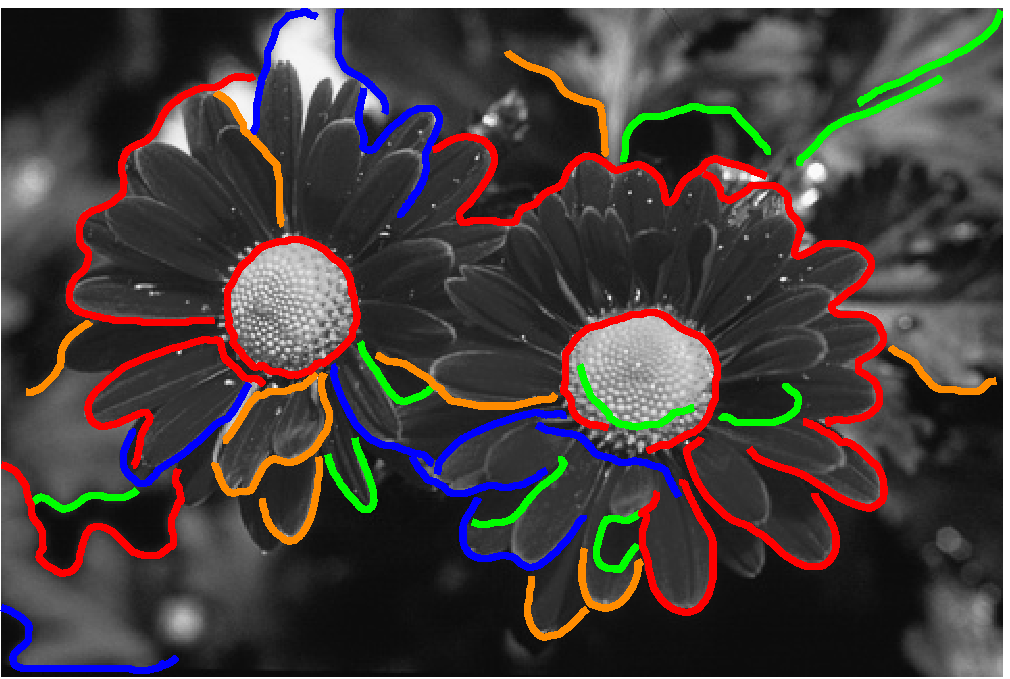
\includegraphics[width=0.24\linewidth]{figs/124084_cons_stats.pdf} &
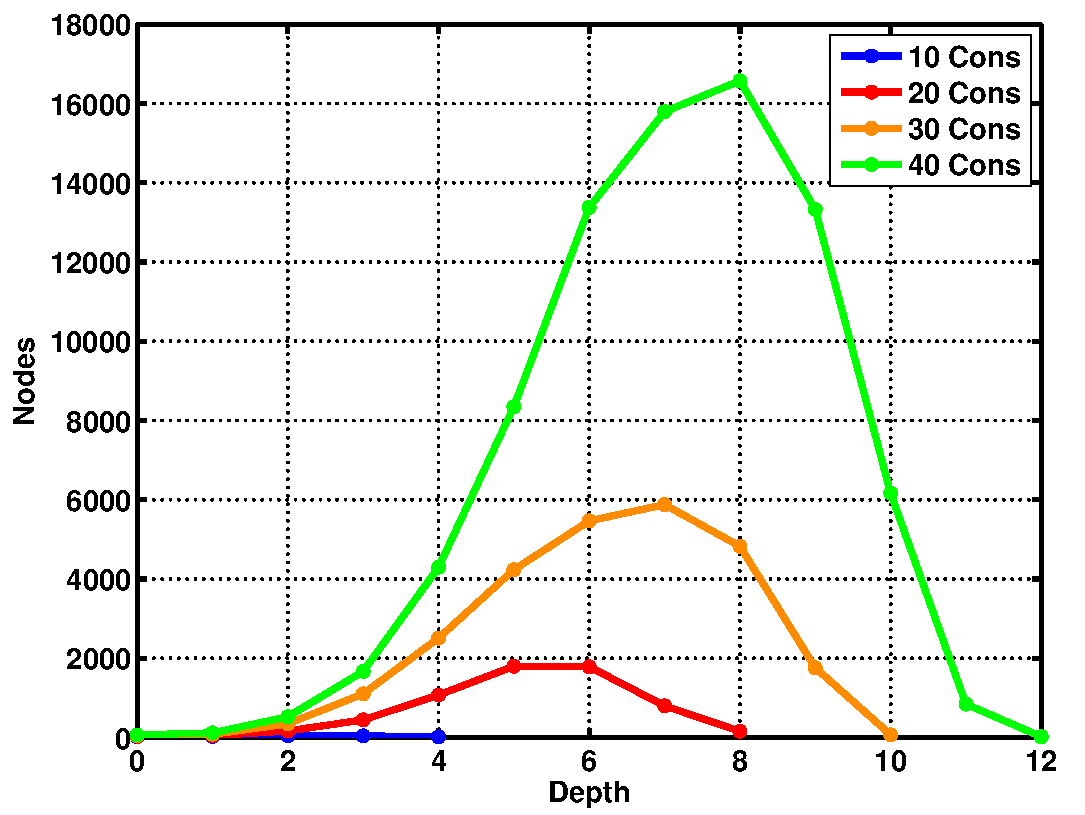
\includegraphics[width=0.24\linewidth]{figs/124084_stats.pdf} &
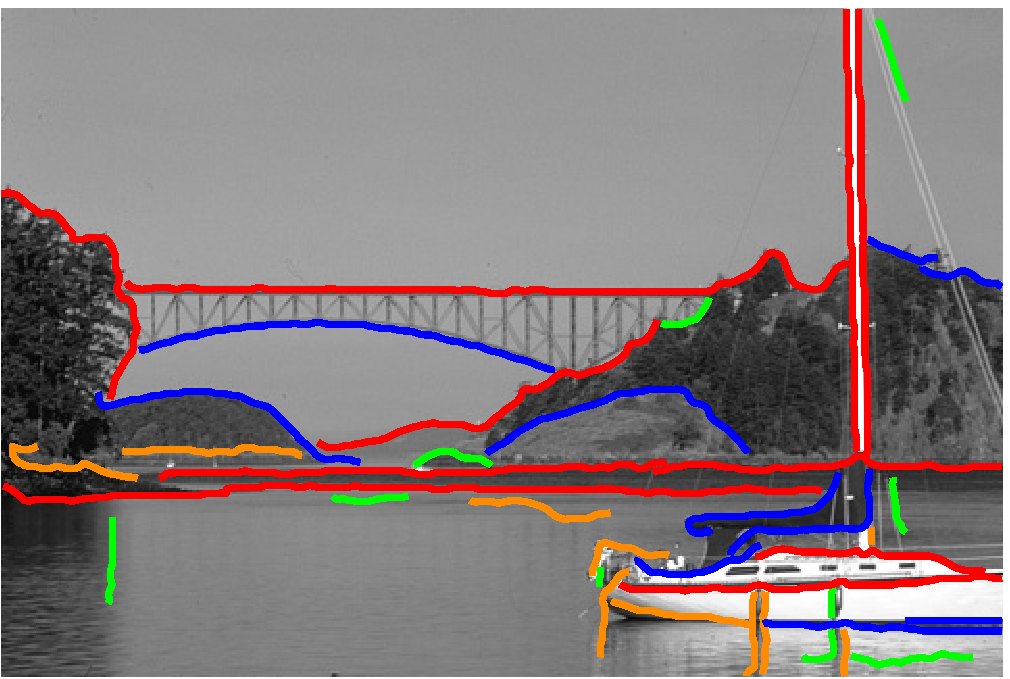
\includegraphics[width=0.24\linewidth]{figs/22090_cons_stats.pdf} &
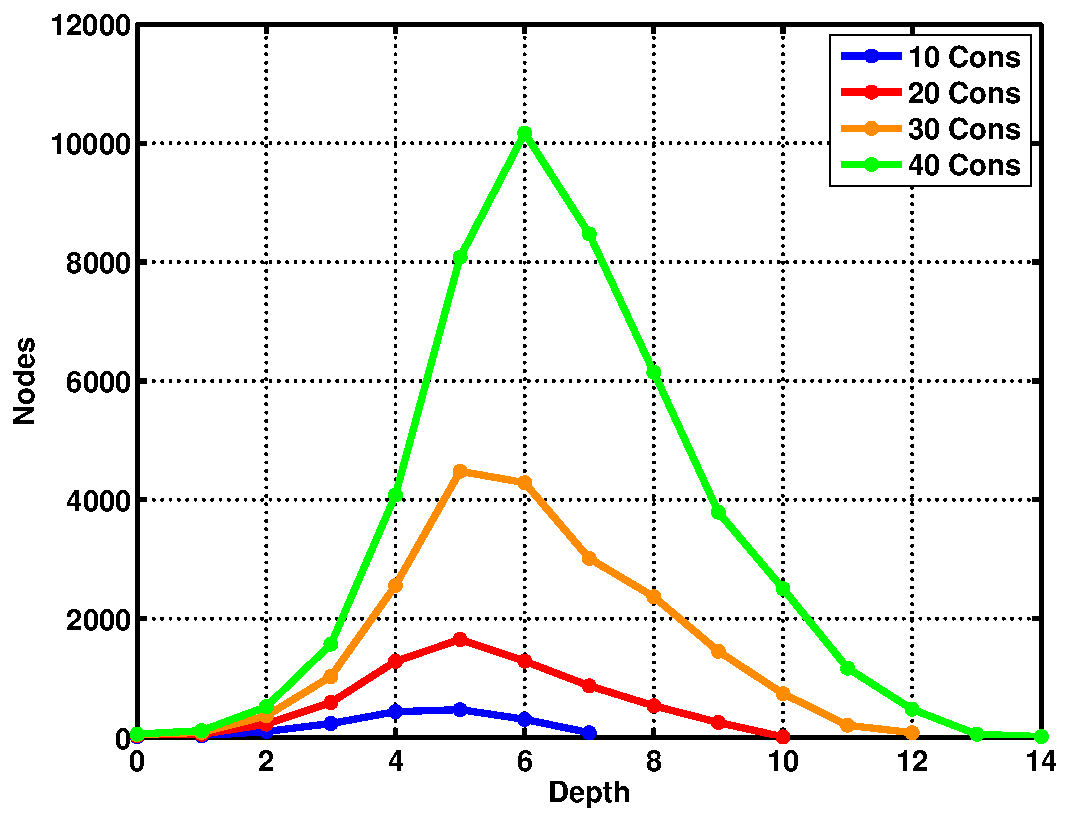
\includegraphics[width=0.24\linewidth]{figs/22090_stats.pdf} \\
\hline
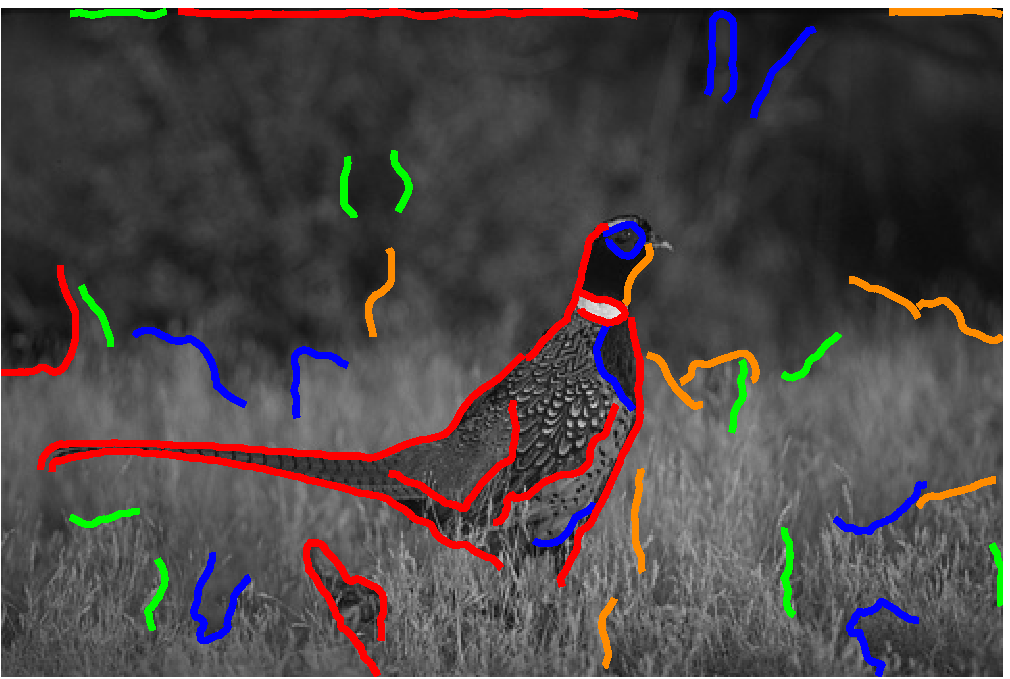
\includegraphics[width=0.24\linewidth]{figs/43074_cons_stats.pdf} &
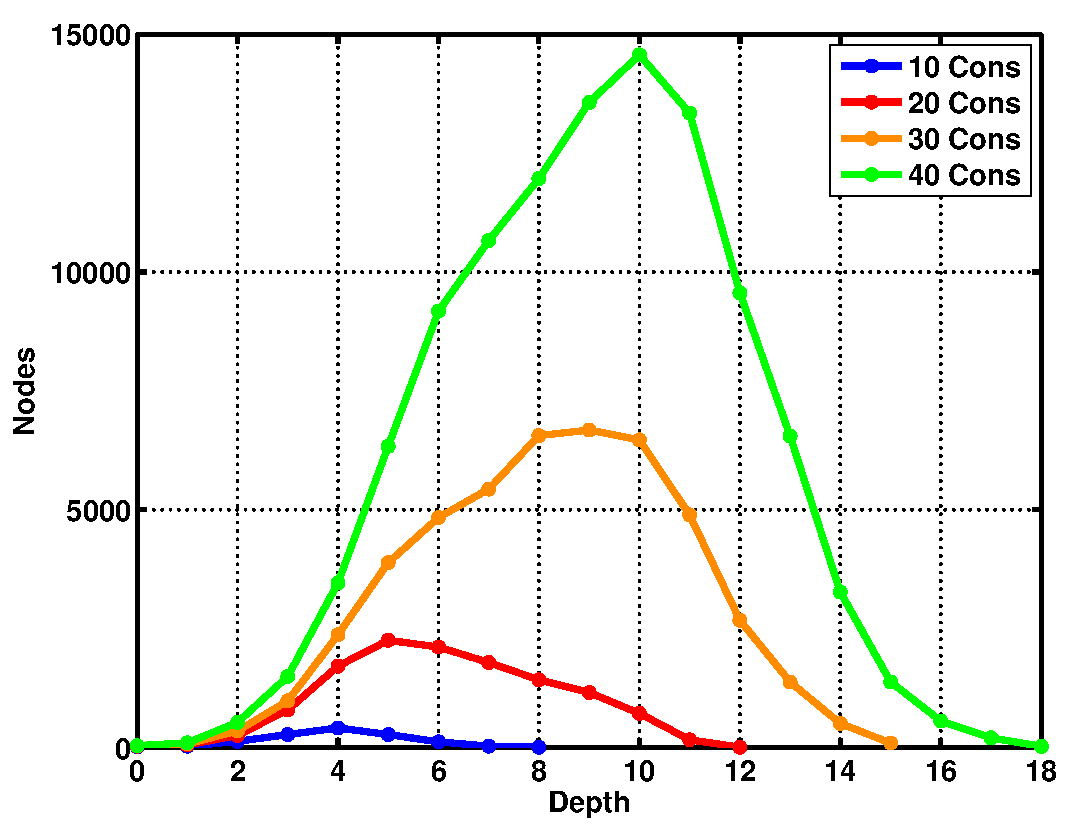
\includegraphics[width=0.24\linewidth]{figs/43074_stats.pdf} &
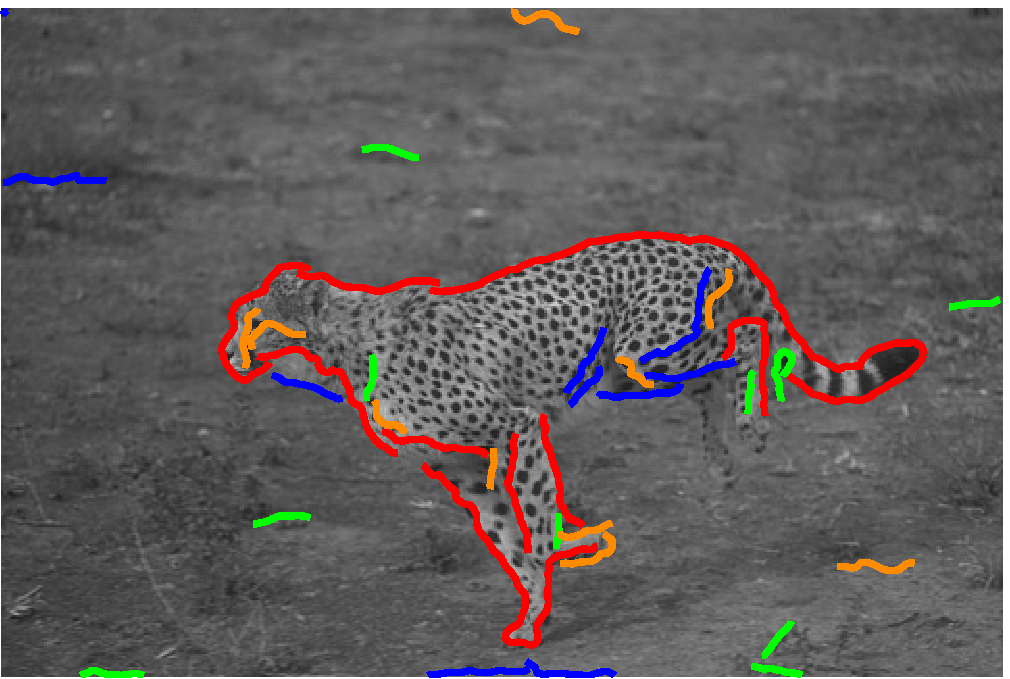
\includegraphics[width=0.24\linewidth]{figs/134008_cons_stats.pdf} &
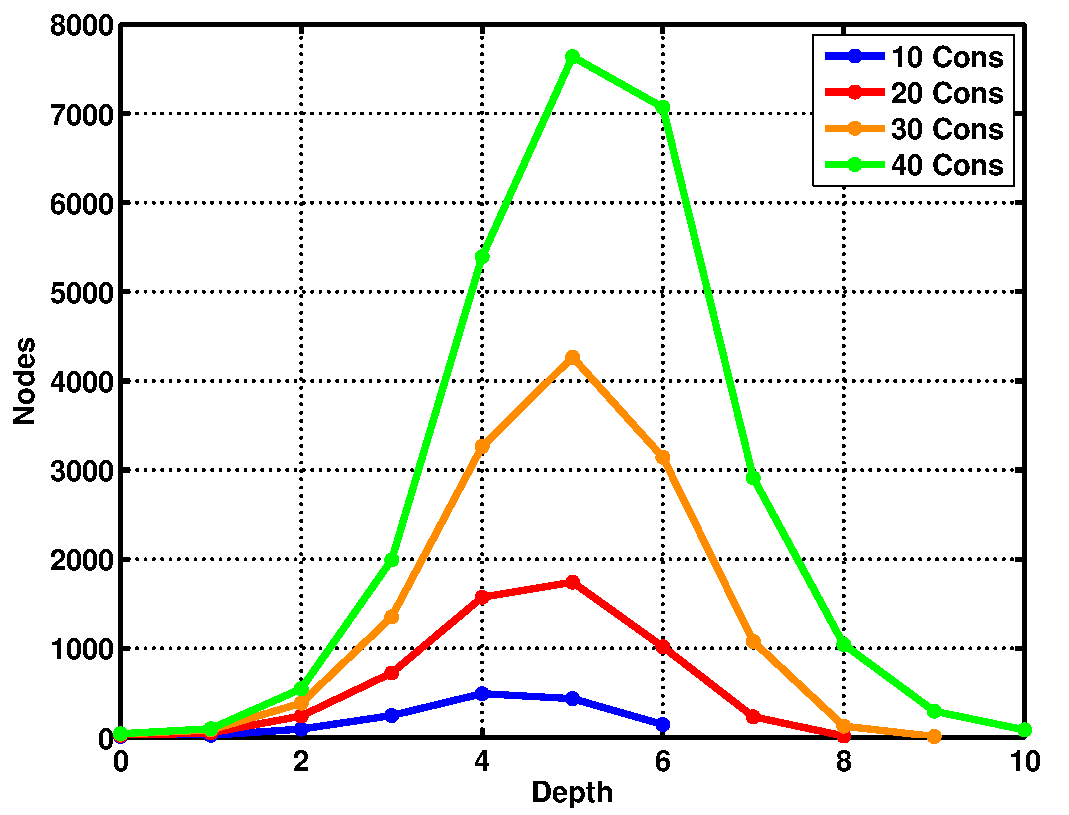
\includegraphics[width=0.24\linewidth]{figs/134008_stats.pdf} \\
\hline
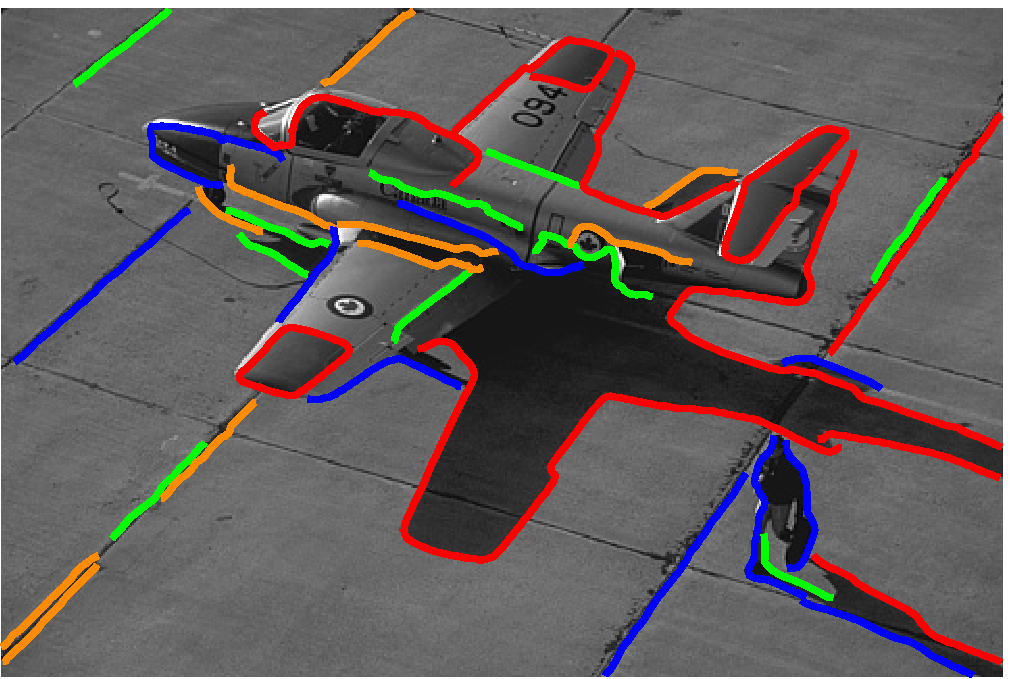
\includegraphics[width=0.24\linewidth]{figs/37073_cons_stats.pdf} &
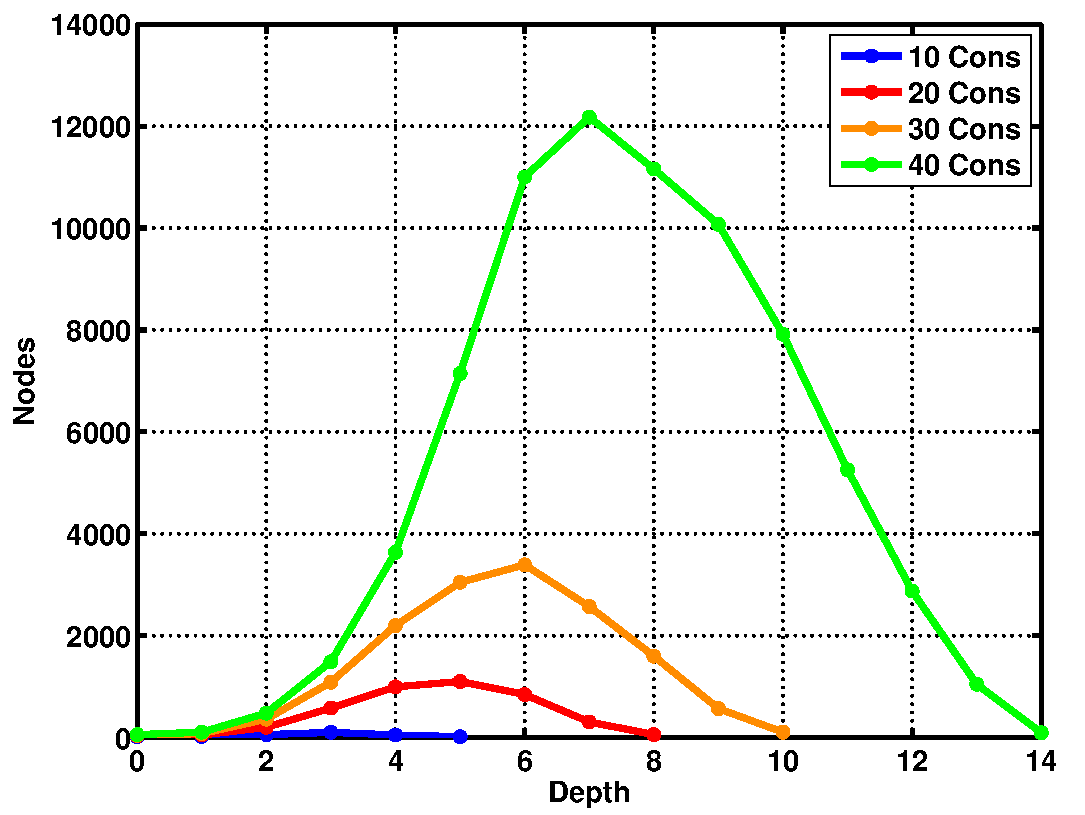
\includegraphics[width=0.24\linewidth]{figs/37073_stats.pdf} &
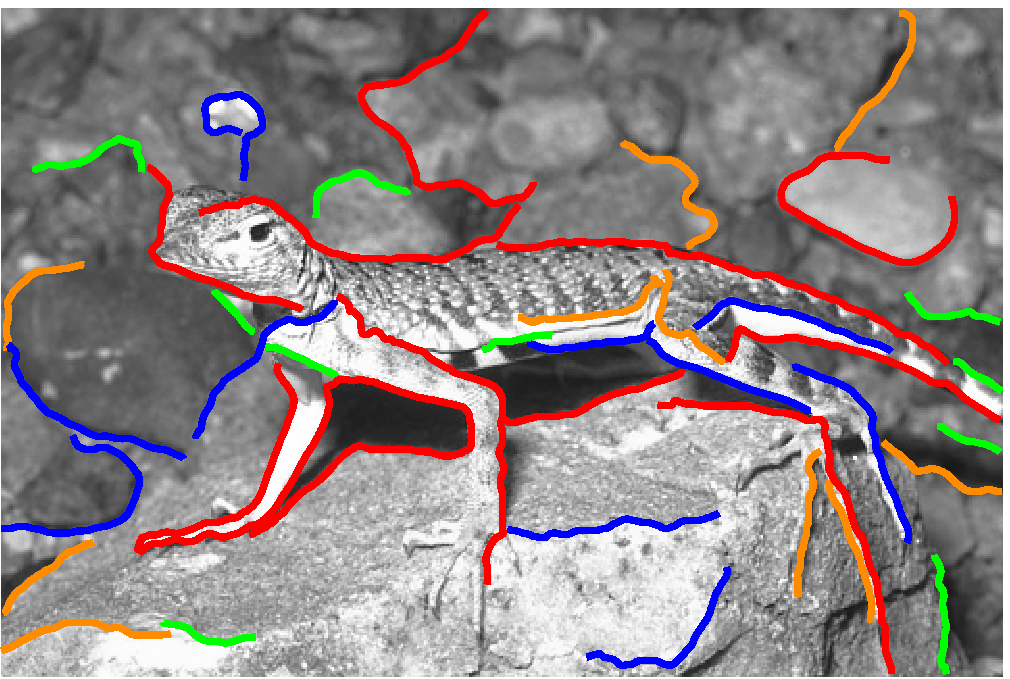
\includegraphics[width=0.24\linewidth]{figs/87046_cons_stats.pdf} &
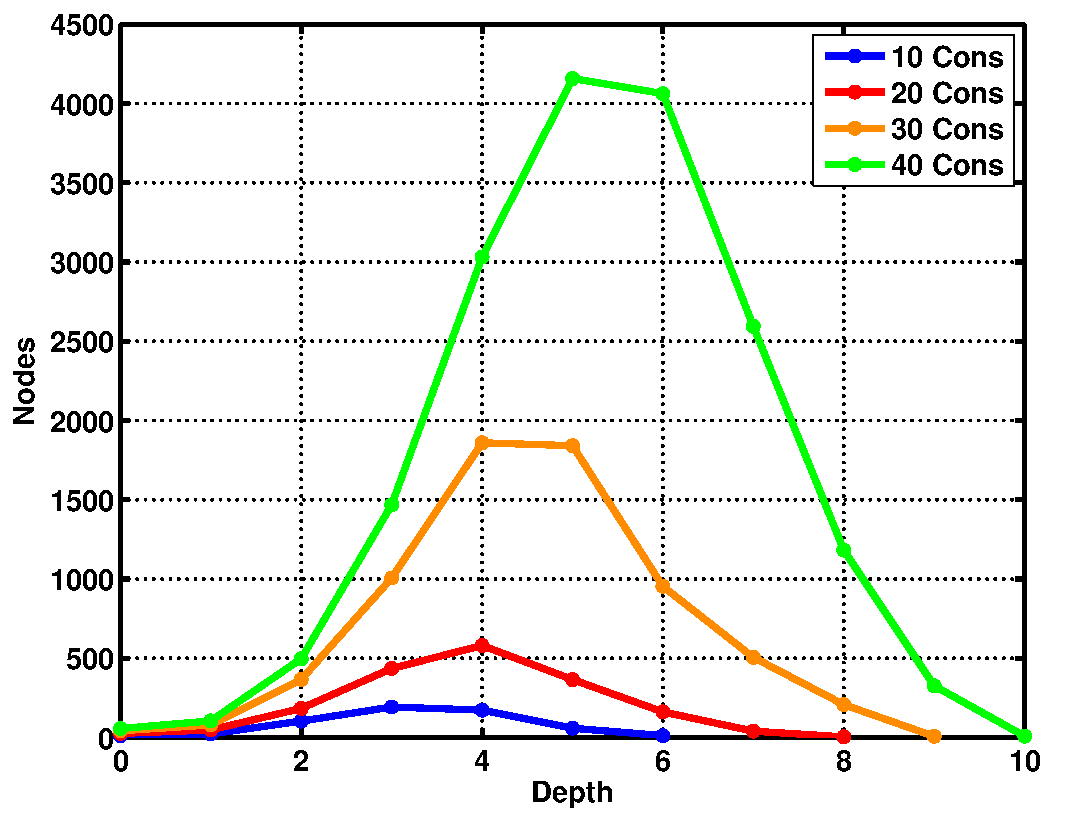
\includegraphics[width=0.24\linewidth]{figs/87046_stats.pdf} \\
\hline
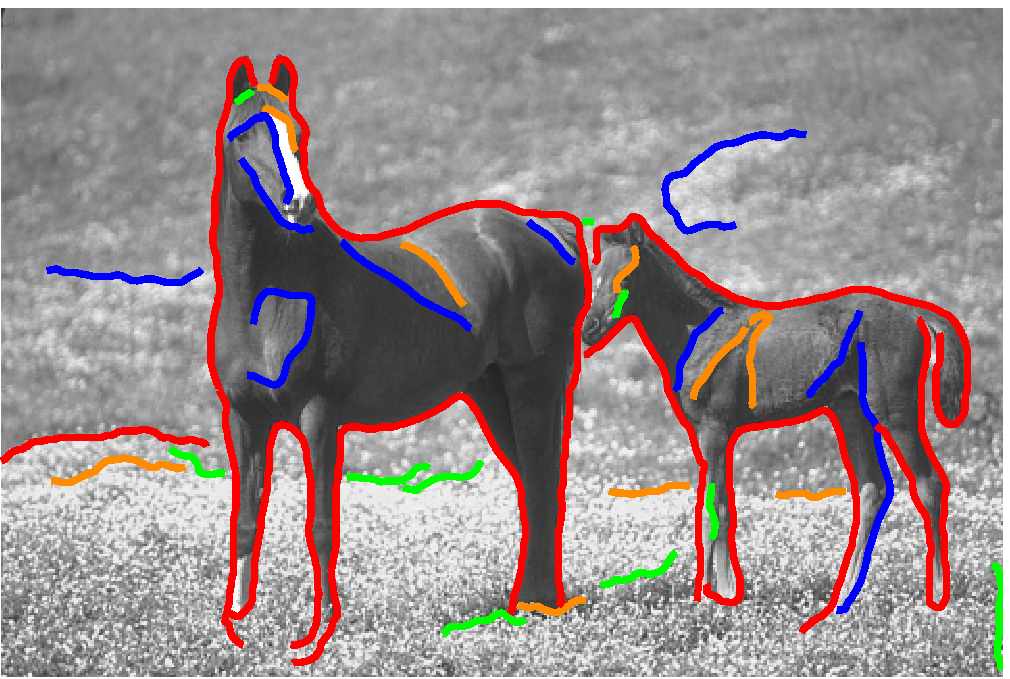
\includegraphics[width=0.24\linewidth]{figs/113016_cons_stats.pdf} &
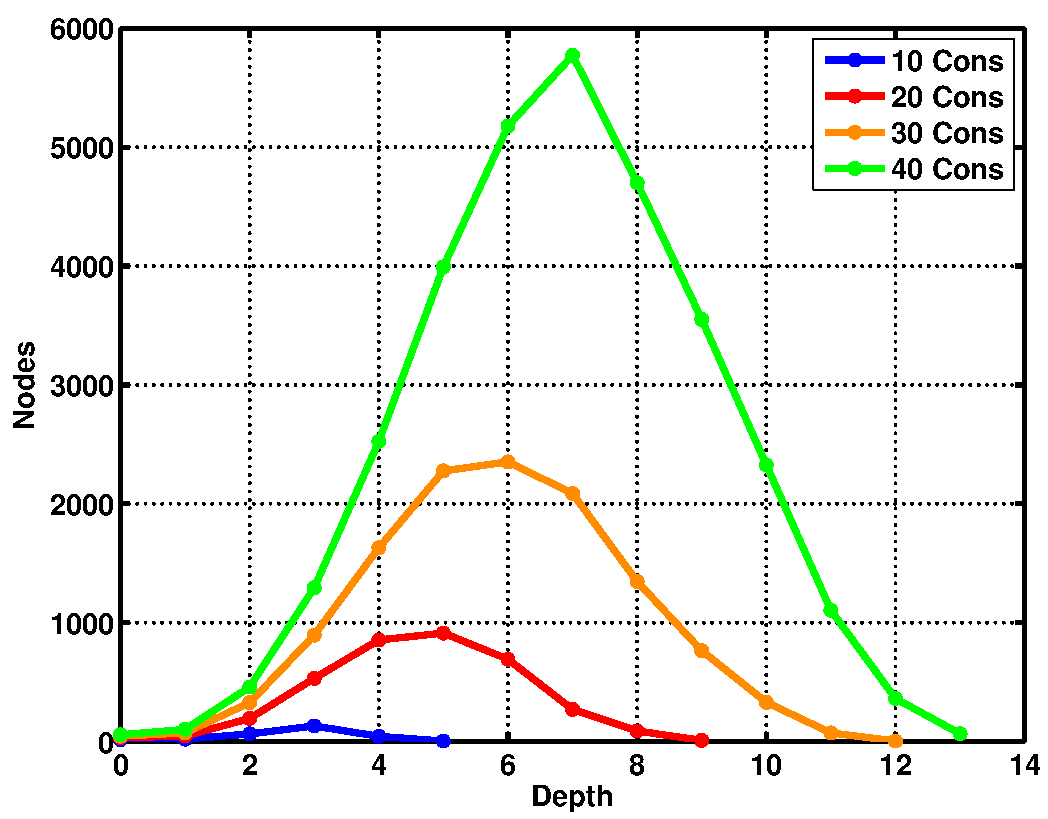
\includegraphics[width=0.24\linewidth]{figs/113016_stats.pdf} &
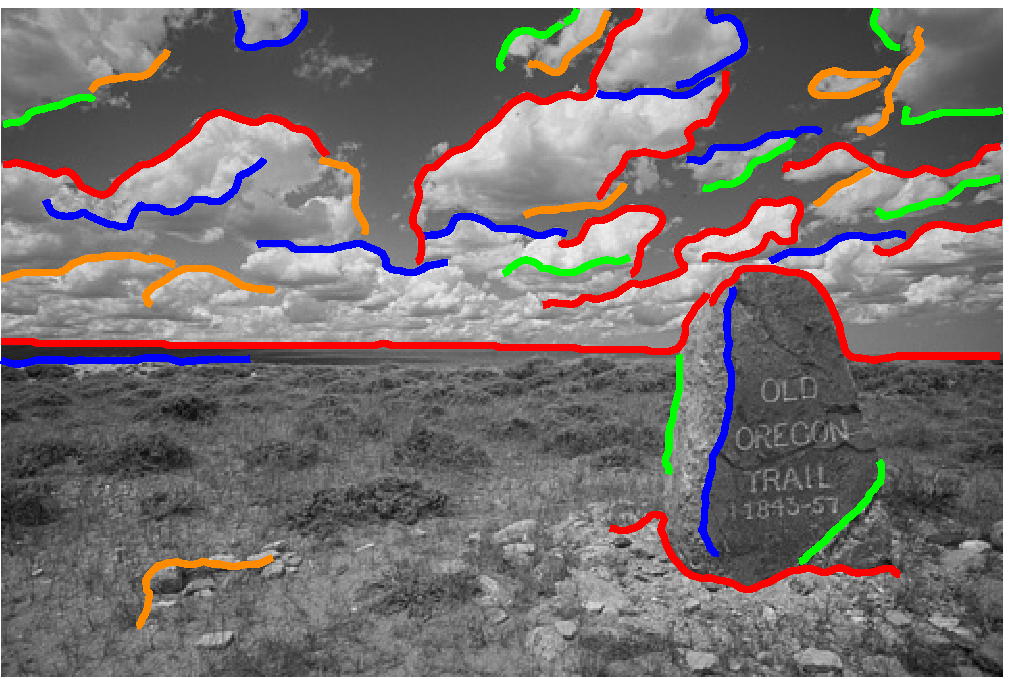
\includegraphics[width=0.24\linewidth]{figs/216066_cons_stats.pdf} &
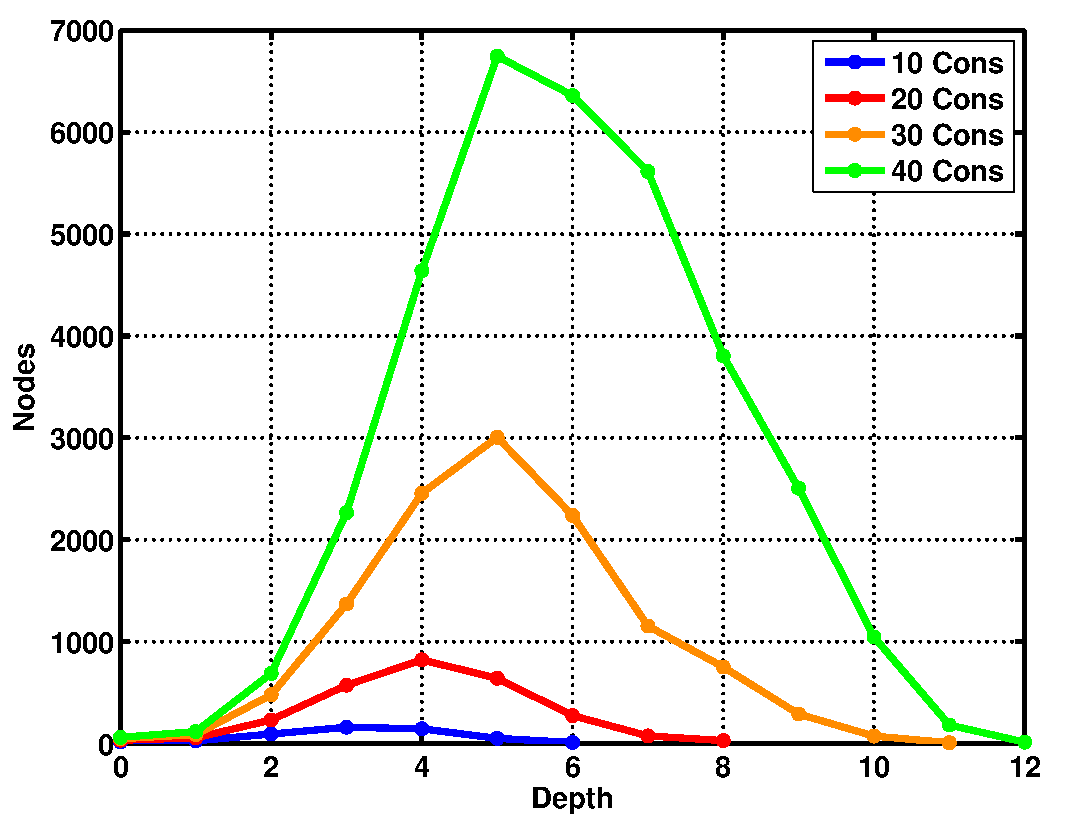
\includegraphics[width=0.24\linewidth]{figs/216066_stats.pdf} \\
\hline
\end{tabular}
\caption{The relationship between the number of nodes in our search space versus the number of contours in an image.  Each image is overlaid with 40 contours (green), 30 contours (orange), 20 contours (red), and 10 contours (blue). Observe how the growth of the search space irrespective of the number of contours reaches a peak and then starts decreasing. This reflects that the various groupings options have been exhausted and no new transform or transform sequences have developed. We observe that this peak shifts as the number of contours are increased.}
\label{fig:cgraph_growth}
\end{figure*}

We empirically measured the size of the containment graph as a function of the number of contour fragments, Figure~\ref{fig:cgraph_growth}. Observe that the expected experimental growth is curtailed, and the containment graph begins to diminish after an initial exponential growth. This ``barrel shaped'' containment graph is typical and is universally observed, as exemplified by a few images. Note that the peak occurs at various depths, typically 5-10 for 40 initial contours. We measure the size of the containment graph, \ie, the area under curves show in Figure~\ref{fig:cgraph_growth}, as modeled by fitting a curve which estimates the size of the containment graph for any number of initial contour fragments, Figure~\ref{fig:gg_growth}. Observe the rate of growth of the curve limits the number of contours we can practically work with. 



\begin{figure*}[!ht]
\centering
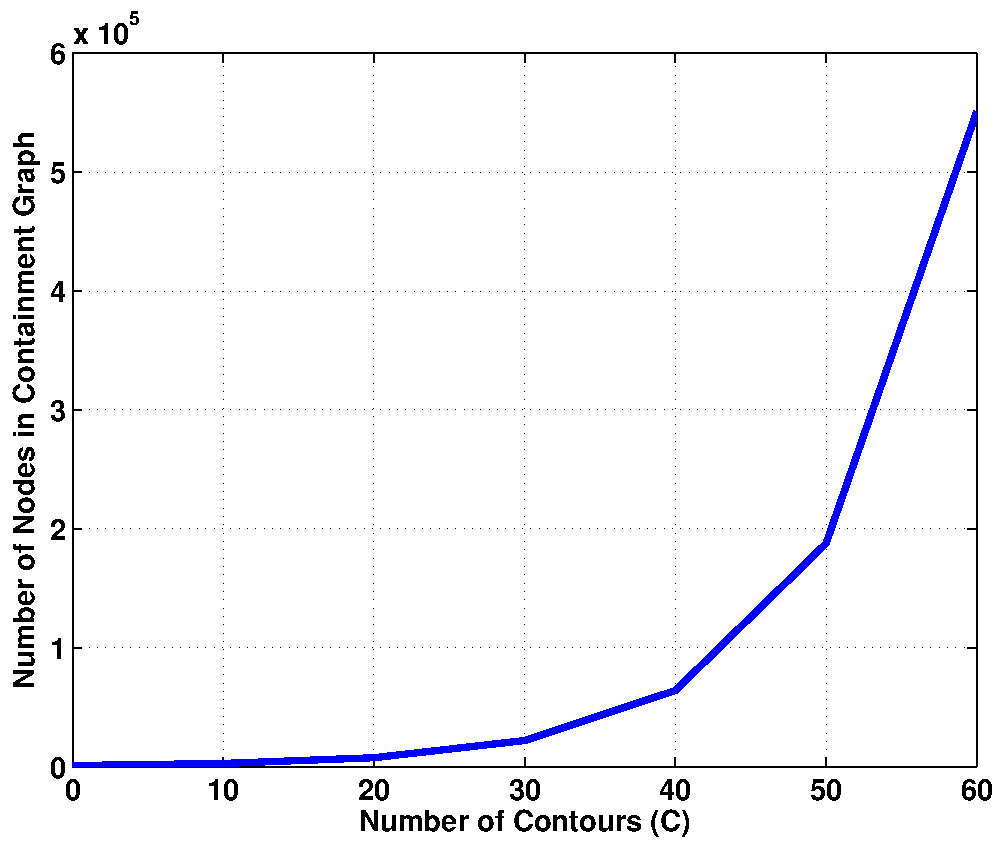
\includegraphics[width=0.32\linewidth]{figs/cgraph_growth.pdf}
%% {\footnotesize\textit{b}}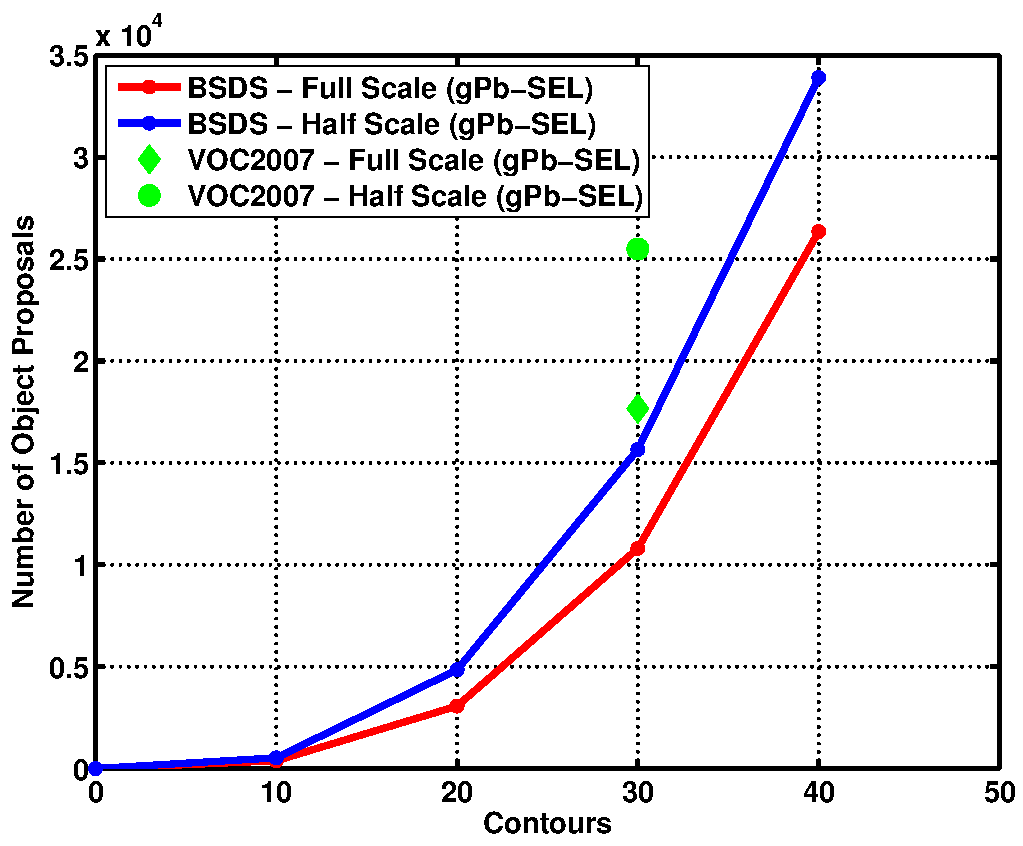
\includegraphics[width=0.47\linewidth]{figs/ops_vs_contours.pdf}
%% {\footnotesize\textit{d}}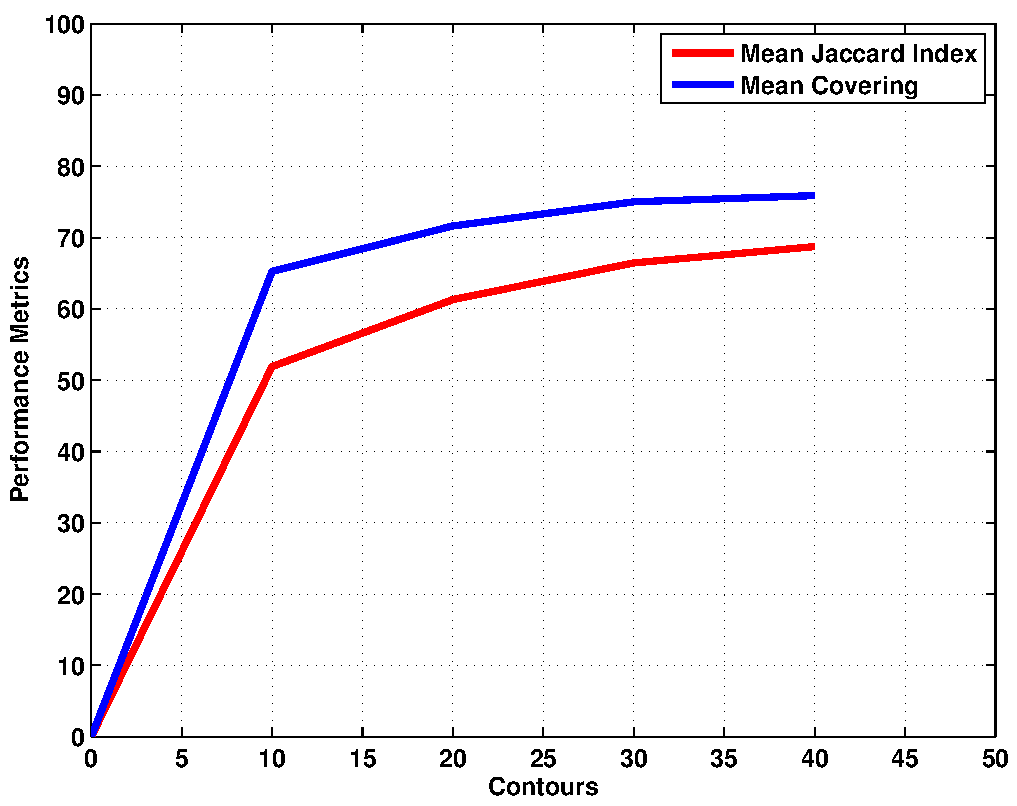
\includegraphics[width=0.47\linewidth]{figs/bsds_performance_vs_contours.pdf}
%% {\footnotesize\textit{e}}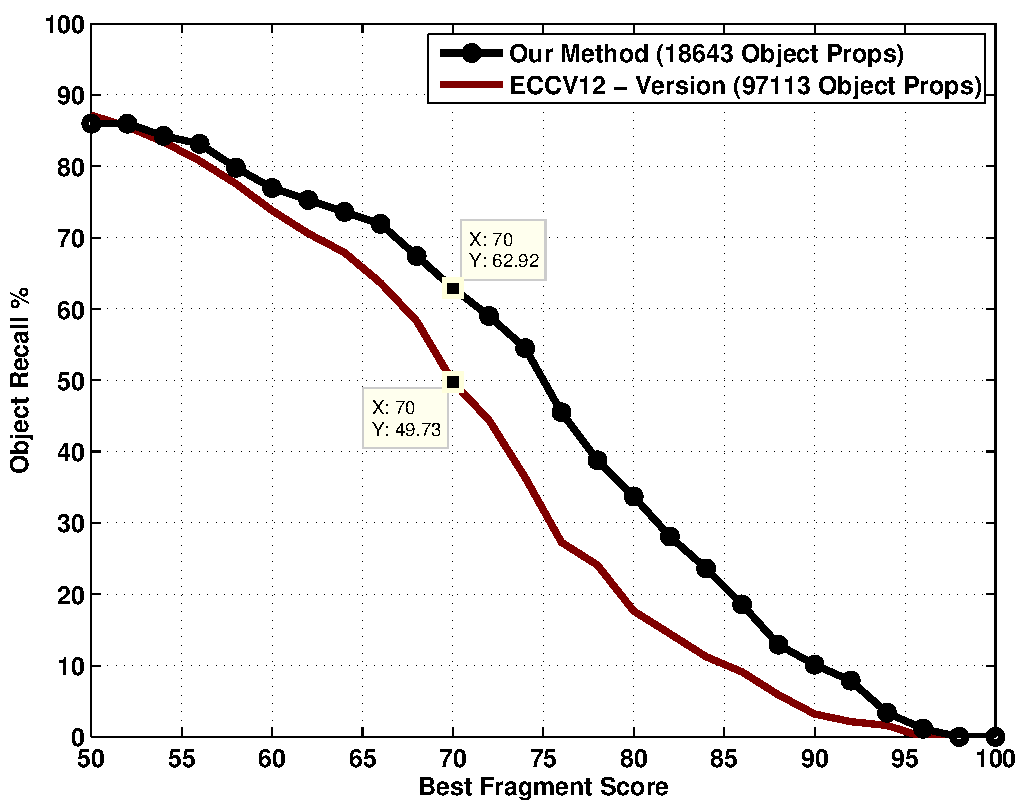
\includegraphics[width=0.47\linewidth]{figs/current_vs_eccv12.pdf}
\caption{We observe an exponential relationship between the number of contours and the size of the containment graph. }
\label{fig:gg_growth}
\end{figure*}

 %% The computational complexity of the system for these settings is measured in Appendix~\ref{sec:cc}.

%% a third-order orientation correction was applied and these edgels were subsequently grouped~\cite{Guo:etal:ECCV14} into contours (ordered set of edgels). The work of ~\cite{Guo:etal:ECCV14} also outputs a probability per contour, which reflects how veridical it is. We rank order all contours and retain the top $N$, on the order of 40-50 contours per image, per scale.  

%% Our search strategy begins with an initial set of seeds. As discussed earlier, Seed MVFs are those which are Type 1, and that further have a 


%% Furthermore the Jaccard Index, Equation~\ref{eq:ji}, between two bounding boxes is much more forgiving than quantifying the pixel overlap between two sets of regions which makes it hard to understand the true performance of an region proposal algorithms. 

\noindent\\
{\bf Comparison To Other Algorithms: } As discussed earlier, Section~\ref{sec:rw}, object proposal algorithms localize the objects of interest in a scene with either a bounding box, \emph{window scoring}, or a region mask, \emph{grouping methods}. Our approach falls under the latter and so we  exclusively compare against other \emph{grouping methods}. A recent extensive survey of the field,~\cite{Hosang:etal:PAMI16}, compared both types in an unified fashion by fitting a bounding box to the region-based proposals thus ignoring the underlying region. While this type of approach can be used if the objects are roughly rectangular object such as bottles, mugs, and cars it is not sufficient for rotated versions of these objects or more deformable objects such as animals or plants. We have extensively compared our approach to as many grouping methods as code is available. In all experiments, competing algorithms have been used with their {\bf default settings}. 

\subsection{Evaluation of Full Object Proposals}

The performance of our approach in generating full object proposals is compared with other approaches when using the BSDS, MSRC, and Seg07 (Pascal 2007) datasets in Figure~\ref{fig:bsds_results}, Figures~\ref{fig:msrc_results},and ~\ref{fig:voc_results} respectively, by reporting various metrics in a table, and by plotting the percent recalled, Equation~\ref{eq:abo_recall}, for different values of $\tau$. Our method is highlighted in cyan for all the tables, while the highest performing method for that specific metric is highlighted in yellow. These results are averages over either the total number of images or the total number of objects. For example, in Figure~\ref{fig:bsds_results} which uses BSDS the ``Mean Covering'' and ``Mean Number of Regions'' are averaged over 246, Table~\ref{tbl:datasets}, images in the dataset while the ``Mean Jaccard Index'' or ``Mean Abo'', Column 2, are averaged over the 648 objects in this dataset. 

We quantify the percent recalled in two ways. First, we look at the number of objects recalled for two specific $\tau$ values. Column 2 of all tables captures the number of object recalled with a $\tau$ equal to 50\% overlap. Interpreting column 3 in Figure~\ref{fig:bsds_results} we observe that our method recovers roughly 91 percent of the total number of objects (648) with at least 50\% overlap. While early work in object recognition was reported at 50\% \emph{Jaccard Index} (Pascal criterion), more recently there is general agreement that object proposals are effective in object recognition when they agree with the ground-truth objects at a higher jaccard index criteria. The accepted $\tau$ level in the literature is at least 70\% BFS, Equation~\ref{eq:bfs}, which is tabulated in Column 3. Secondly, we show the full curve alongside each table, where $\tau$ of 50\% and 70\% represent two samples of the full curve. 

It is important to understand all these performance metrics with respect to the size of the pool of object candidates, Column 5 of Tables. A method that achieves a higher $covering$ or $ABFS$ with a fewer number of segments has better focused its results on true object regions. Intuitively, the larger the pool of object candidates the greater the likelihood of capturing true object or part regions at the expense of an increase in the number of non-veridical regions. This trade-off between efficiency and maximizing performance is an important dimension in comparing varying object proposal algorithms. 

%% In summary, we asses the performance of our work and any competing algorithms according to four metrics: $Covering$,$ABFS$,$Object$ $Recall$ or \emph{Part Recall}, and finally the number of candidate object proposals.

\begin{figure*}[ht]
\begin{center}
\scriptsize
\begin{tabular}{ |l|P{1.1cm}|P{0.8cm}|P{0.8cm}|P{1.1cm}|P{1.27cm}| }
\hline
\multicolumn{6}{|c|}{BSDS300 Test+Train Set annotated by~\cite{Endres:Hoiem:PAMI14}}\\
\hline
Method & Mean Jaccard Index & Recall @ 50(\%) & Recall @ 70(\%) & Mean Covering & Mean Number Regions\\
\hline
MCG~\cite{Arbelaez:etal:CVPR14} &  \cellcolor{yellow}{76.66} &  \cellcolor{yellow}{91.67} &  \cellcolor{yellow}{73.30} &  \cellcolor{yellow}{81.25} & 4198.33 \\
\hline
\rowcolor{cyan} {\bf Our Method} & {\bf  74.34} & {\bf  91.05} & {\bf  69.60} & {\bf  79.40} & {\bf 5441.39} \\
\hline
LPO~\cite{Krahenbuhl:Koltun:CVPR15} &  71.29 &  88.58 &  60.19 &  76.63 & \cellcolor{yellow}{558.02} \\
\hline
Rigor~\cite{Humayun:etal:CVPR14} &  70.46 &  83.33 &  62.96 &  78.88 & 1126.70 \\
\hline
GOP~\cite{Krahenbuhl:Koltun:ECCV14} &  67.83 &  86.57 &  52.01 &  73.21 & 743.28 \\
\hline
Rantalankila~\cite{Rantalankila:etal:CVPR14} &  66.09 &  78.24 &  51.39 &  75.20 & 1559.33 \\
\hline
CPMC~\cite{Carreira:Sminchisescu:PAMI12} &  64.96 &  76.85 &  52.01 &  74.53 & 599.88 \\
\hline
CIP~\cite{Endres:Hoiem:PAMI14} &  64.15 &  75.93 &  48.61 &  72.10 & 1258.17 \\
\hline
Shape Sharing~\cite{Kim:Grauman:ECCV12} &  63.40 &  73.46 &  52.78 &  75.20 & 1107.43 \\
\hline
gPb-owt-ucm~\cite{Arbelaez:etal:PAMI11} &  60.01 &  66.20 &  32.72 &  61.94 & 2491.21 \\
\hline
\end{tabular}
\raisebox{-0.5\height}{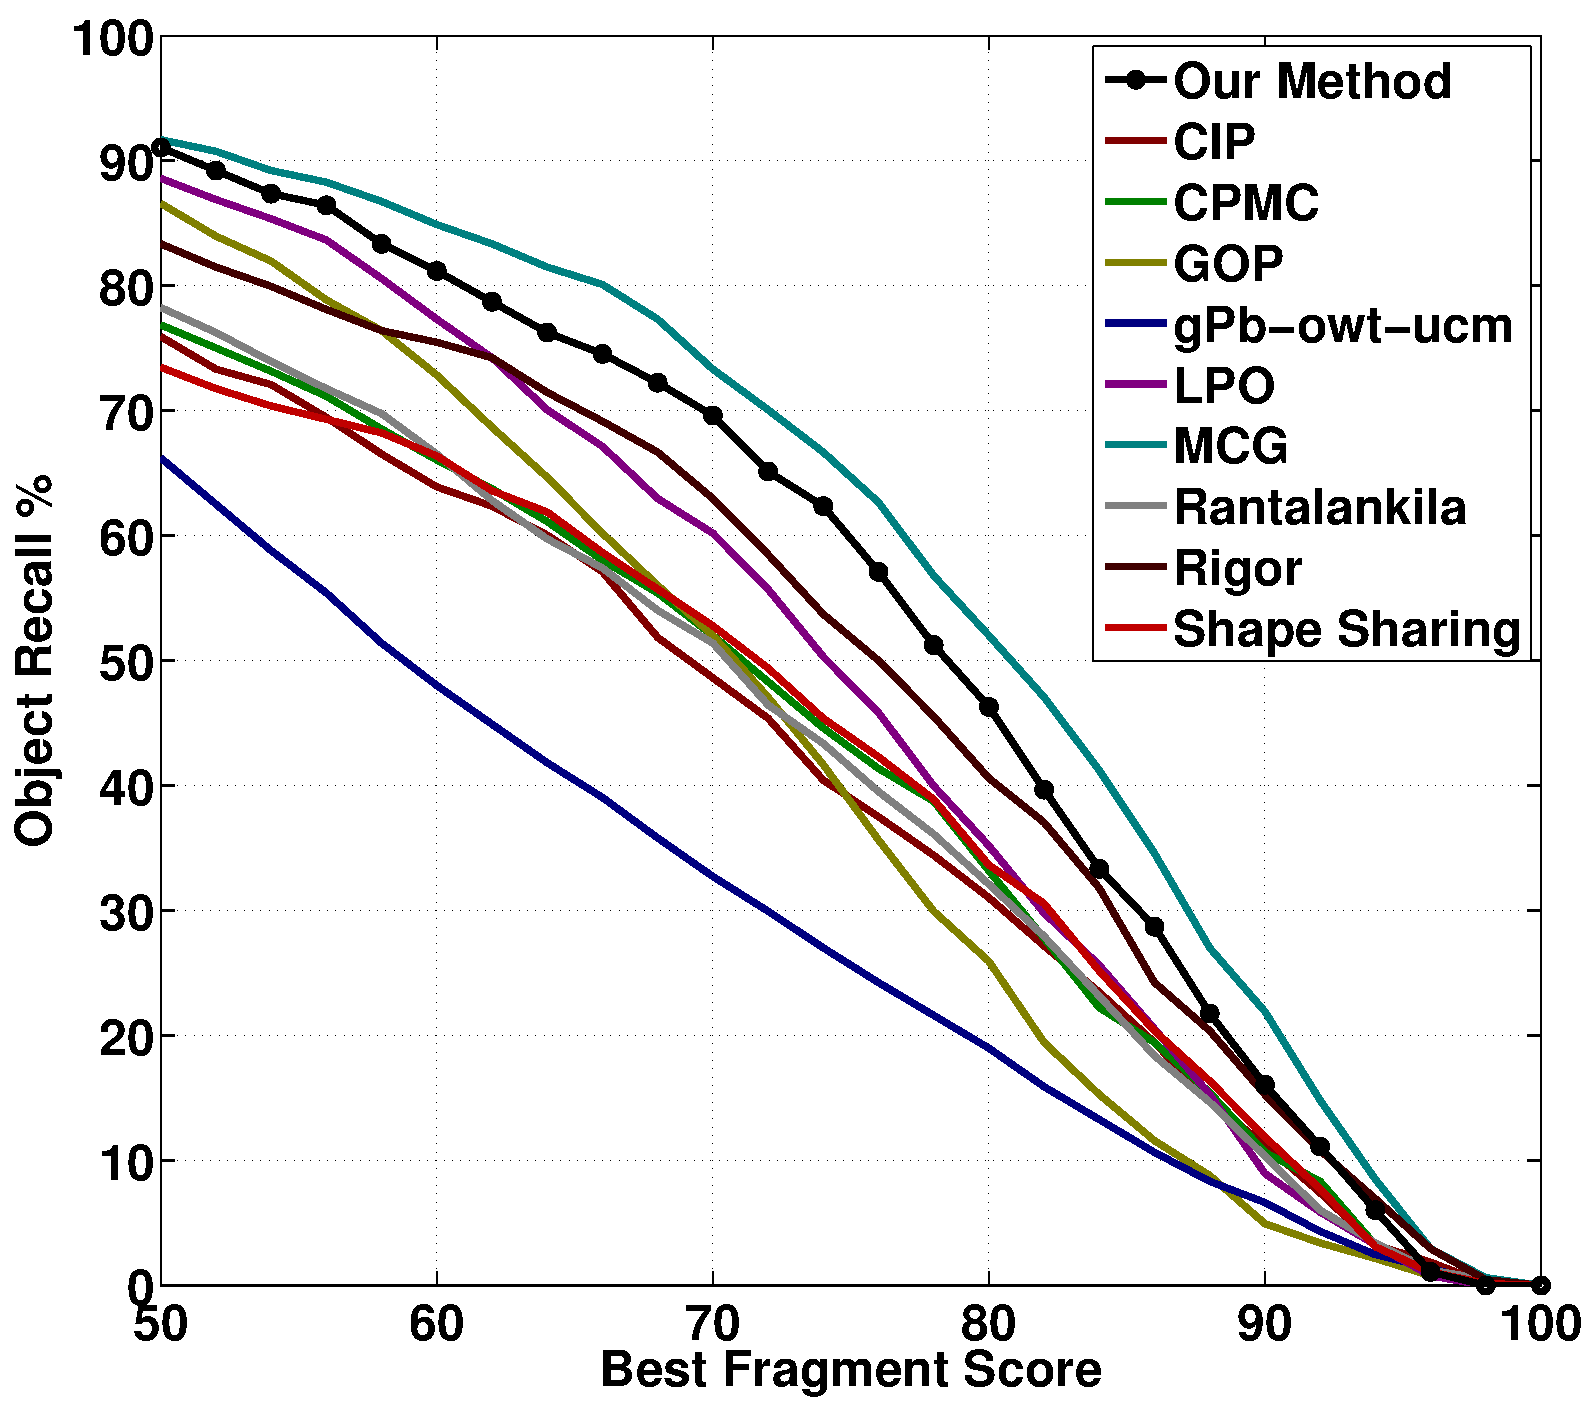
\includegraphics[width=0.34\textwidth]{figs/bsds_object_recall.pdf}}
\end{center}
\vspace{-0.5cm}
\caption{Table: We evaluate our approach on BSDS as labeled by~\cite{Endres:Hoiem:PAMI14} using various metrics. Notice how our results, highlighted in \textcolor{cyan}{cyan}, are very close to the top performing method. Graph: The object recall curve highlights the percentage of objects recalled for a fixed BFS.}
\label{fig:bsds_results} 
\end{figure*}

\begin{figure*}[ht]
\begin{center}
\scriptsize
\begin{tabular}{ |l|P{1.1cm}|P{0.8cm}|P{0.8cm}|P{1.1cm}|P{1.27cm}| }
\hline
\multicolumn{6}{|c|}{ MSRC annotated by~\cite{Malisiewicz:Efros:BMVC07}}\\
\hline
Method & Mean Jaccard Index & Recall @ 50(\%) & Recall @ 70(\%) & Mean Covering & Mean Number Regions\\
\hline
MCG~\cite{Arbelaez:etal:CVPR14} &  \cellcolor{yellow}{83.92} &  \cellcolor{yellow}{97.81} &  \cellcolor{yellow}{87.97} &  87.96 & 4191.76 \\
\hline
\rowcolor{cyan} {\bf Our Method} & {\bf  83.06} & {\bf  97.59} & {\bf  87.81} & {\bf  85.92} & {\bf 5643.27} \\
\hline
Rantalankila~\cite{Rantalankila:etal:CVPR14} &  81.75 &  95.14 &  83.22 &  \cellcolor{yellow}{87.99} & 905.73 \\
\hline
Rigor~\cite{Humayun:etal:CVPR14} &  81.47 &  94.33 &  82.36 &  87.74 & 863.73 \\
\hline
CPMC~\cite{Carreira:Sminchisescu:PAMI12} &  81.08 &  93.69 &  83.16 &  87.24 & \cellcolor{yellow}{448.24} \\
\hline
CIP~\cite{Endres:Hoiem:PAMI14} &  79.01 &  92.25 &  78.93 &  86.66 & 563.94 \\
\hline
Shape Sharing~\cite{Kim:Grauman:ECCV12} &  78.48 &  91.55 &  78.17 &  83.75 & 898.27 \\
\hline
GOP~\cite{Krahenbuhl:Koltun:ECCV14} &  78.04 &  95.62 &  77.61 &  82.21 & 746.46 \\
\hline
LPO~\cite{Krahenbuhl:Koltun:CVPR15} &  77.34 &  94.23 &  73.86 &  81.88 & 528.42 \\
\hline
gPb-owt-ucm~\cite{Arbelaez:etal:PAMI11} &  73.99 &  84.23 &  62.37 &  78.50 & 1112.91 \\
\hline
\end{tabular}
\raisebox{-0.5\height}{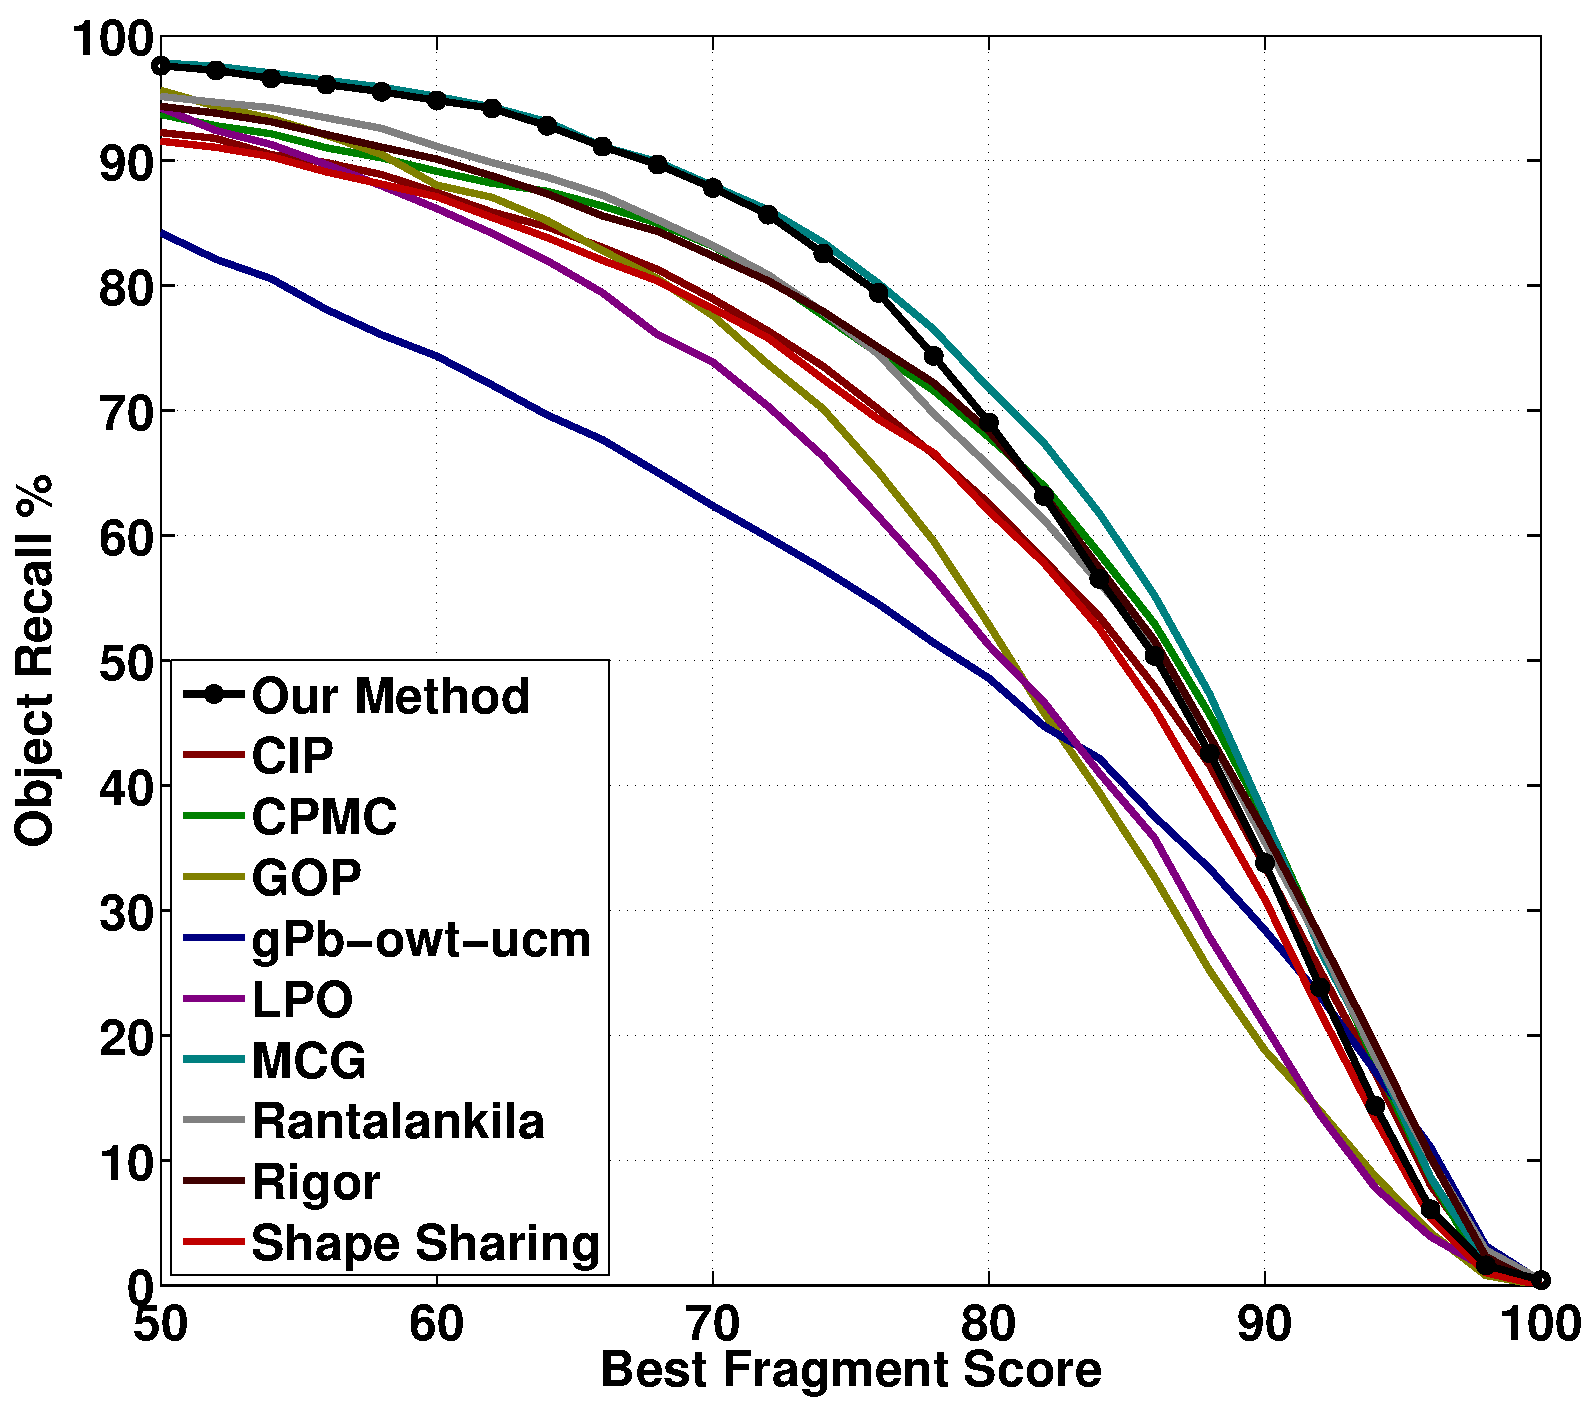
\includegraphics[width=0.34\textwidth]{figs/msrc_object_recall.pdf}}
\end{center}
\vspace{-0.5cm}
\caption{Table: We evaluate our approach on MSRC~\cite{malisiewicz:bmvc07} using various metrics. Notice how our results, highlighted in \textcolor{cyan}{cyan}, are very close to the top performing method. Graph: The object recall curve highlights the percentage of objects recalled for a fixed BFS.}
\label{fig:msrc_results}  
\end{figure*}

\begin{figure*}[ht]
\begin{center}
\scriptsize
\begin{tabular}{ |l|P{1.1cm}|P{0.8cm}|P{0.8cm}|P{1.1cm}|P{1.27cm}| }
\hline
\multicolumn{6}{|c|}{ SegVOC07~\cite{pascal-voc-2007}}\\
\hline
Method & Mean Jaccard Index & Recall @ 50(\%) & Recall @ 70(\%) & Mean Covering & Mean Number Regions\\
\hline
MCG~\cite{Arbelaez:etal:CVPR14} &  \cellcolor{yellow}{70.56} &  \cellcolor{yellow}{85.67} &  \cellcolor{yellow}{58.65} &  \cellcolor{yellow}{77.56} & 5622.34 \\
\hline
\rowcolor{cyan} {\bf Our Method} & {\bf  64.02} & {\bf  74.57} & {\bf  49.65} & {\bf  73.94} & {\bf 5734.67} \\
\hline
LPO~\cite{Krahenbuhl:Koltun:CVPR15} &  62.90 &  73.97 &  41.35 &  71.58 & 702.27 \\
\hline
Rigor~\cite{Humayun:etal:CVPR14} &  62.66 &  71.99 &  44.48 &  74.67 & 1451.34 \\
\hline
Rantalankila~\cite{Rantalankila:etal:CVPR14} &  62.09 &  70.68 &  46.46 &  75.39 & 1819.69 \\
\hline
GOP~\cite{Krahenbuhl:Koltun:ECCV14} &  61.50 &  74.14 &  38.06 &  69.60 & 798.21 \\
\hline
CIP~\cite{Endres:Hoiem:PAMI14} &  61.47 &  71.17 &  43.99 &  73.31 & 1814.63 \\
\hline
CPMC~\cite{Carreira:Sminchisescu:PAMI12} &  58.57 &  64.74 &  42.17 &  72.82 & \cellcolor{yellow}{697.26} \\
\hline
Shape Sharing~\cite{Kim:Grauman:ECCV12} &  58.57 &  63.43 &  51.40 &  76.57 & 1142.43 \\
\hline
gPb-owt-ucm~\cite{Arbelaez:etal:PAMI11} &  54.35 &  54.37 &  21.58 &  57.54 & 2414.51 \\
\hline
\end{tabular}
\raisebox{-0.5\height}{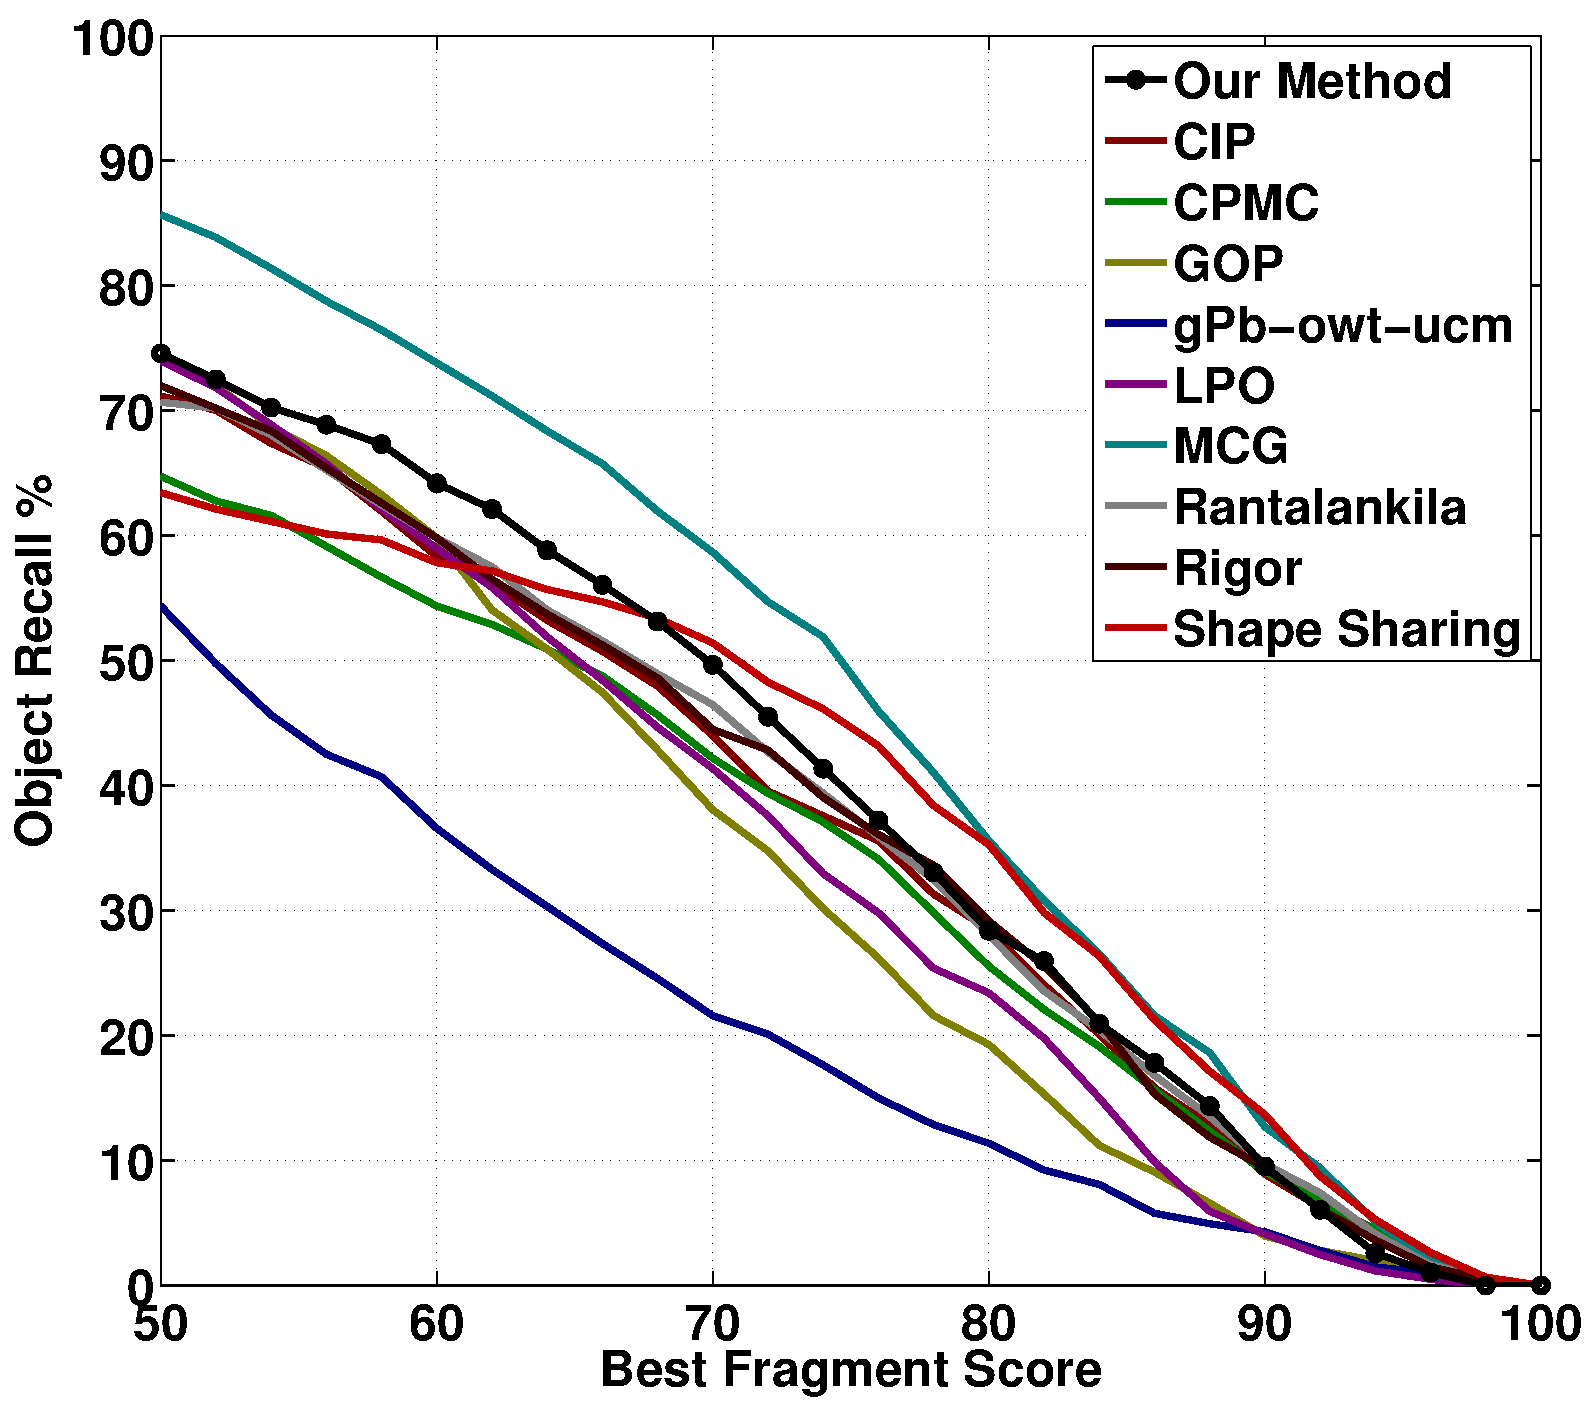
\includegraphics[width=0.34\textwidth]{figs/voc2007_object_recall.pdf}}  
\end{center}
\vspace{-0.5cm}
\caption{Table: We evaluate our approach on the PASCAL VOC 2007 dataset using various metrics. Notice how our results, highlighted in \textcolor{cyan}{cyan}, are very close to the top performing method. Graph: The object recall curve highlights the percentage of objects recalled for a fixed BFS.}
\label{fig:voc_results}
\end{figure*}


\noindent\\

We observe the performance of our approach is state of the art across all the metrics. Observe that the performance of our bottom-up approach exceeds the two top-down learning methods, LPO~\cite{Krahenbuhl:Koltun:CVPR15}  and Shape Sharing~\cite{Kim:Grauman:ECCV12}. Also, observe from the object recall curve that our method and MCG~\cite{Arbelaez:etal:CVPR14} are set apart from the remaining methods. We note that our method performs significantly better on BSDS and MSRC compared to VOC2007. This is mainly because the more complex scenes of VOC2007 have relatively more contour content, and the maximum number of contours that we can process with our current implement is 60 contours ( this limit can be significantly alleviated with a more efficient implementation ).  Figures~\ref{fig:bsds_examples},~\ref{fig:msrc_examples}, and ~\ref{fig:voc_results} depict example outputs of our system on this dataset showing the image, ground-truth annotation, and our output. In the last column, each ground-truth object has been overlaid with our best matching object proposal along with a textual annotation of the Jaccard Index.

%% {\bf BSDS (Figure~\ref{fig:bsds_results}):} We observe that our performance irrespective of metric is state of the art. While most of the methods are purely bottom-up we observe that our performance exceeds  If we look at our object recall curve, black dotted curve, we notice our method and MCG~\cite{Arbelaez:etal:CVPR14} are separated from the rest of the methods.  Example outputs of our system on this dataset can be seen in 

%% \noindent\\
%% {\bf MSRC (Figure~\ref{fig:msrc_results}):} We observe that our performance irrespective of metric is state of the art. While most of the methods are purely bottom-up we observe that our performance exceeds top-down learning methods, LPO~\cite{Krahenbuhl:Koltun:CVPR15} and Shape Sharing~\cite{Kim:Grauman:ECCV12}. If we look at our object recall curve, black dotted curve, we notice for all various $BFS$ levels it bounds other methods. Example outputs of our system can be seen in Figure~\ref{fig:msrc_examples} where we have shown the image, ground-truth annotation, and our output. In the last column, each ground-truth object has been overlaid with our best matching object proposal along with a textual annotation of the Jaccard Index.

%% \noindent\\
%% {\bf VOC2007 (Figure~\ref{fig:voc_results}):} Compared to the other datasets our performance suffers on this dataset. Due to computational reasons we restrict the number of contours (40-60) we can process. The scenes in VOC2007 are much more complex (more objects, occlusion, \etc), however, requiring on the order of 100-200 contours. Example outputs of our system can be seen in Figure~\ref{fig:voc_examples} where we have shown the image, ground-truth annotation, and our output. In the last column, each ground-truth object has been overlaid with our best matching object proposal along with a textual annotation of the Jaccard Index.

Overall, if we compare our results versus other methods we see that in general our approach is right behind MCG~\cite{Arbelaez:etal:CVPR14} irrespective of the comparison metric used. Note that our input is  globalPb ({\it gPb})~\cite{Maire:etal:CVPR08}, the same used by MCG~\cite{Arbelaez:etal:CVPR14}. In both methods, the performance is comparable as both are dependent on the quality and/or errors of the \emph{gPb} input. The key difference between our approach and MCG is how-scale is handled.  Their algorithm runs the gpb-owt-ucm~\cite{Arbelaez:etal:PAMI11} algorithm at three different scales, and the region hierarchies are then aligned across scales into one unified region hierarchy. The paper shows that this multi-scale approach leads to huge improvements in the performance of the system. In our case, we instead run across two scales independently and take the union of the results. Given the close performance of our approach to MCG we conjecture that properly integrating scale can lead to dramatic improvements. 




%% Figure~\ref{fig:MSRC} shows the best fragment per annotated object for a selection from MSRC images with a comparison to~\cite{Carreira:Sminchisescu:PAMI12,Arbelaez:etal:CVPR09}. 
%% \noindent
%% Figure~\ref{fig:BSDS} illustrates our results on BSDS with a comparison to~\cite{Endres:Hoiem:ECCV10,Carreira:Sminchisescu:PAMI12}. 

%% \begin{figure}[!h]
%% %\vspace{-0.5cm}
%% \centering
%%  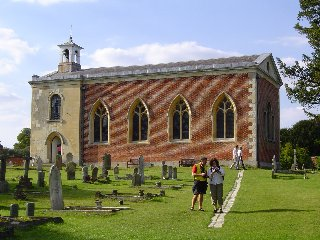
\includegraphics[width=0.15\textwidth]{figs/3_16_s.jpg}
%%   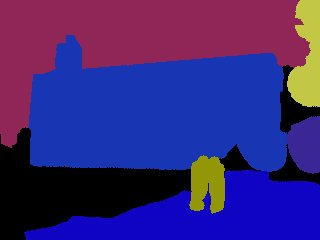
\includegraphics[width=0.15\textwidth]{figs/3_16_s_gt.jpg}
%%    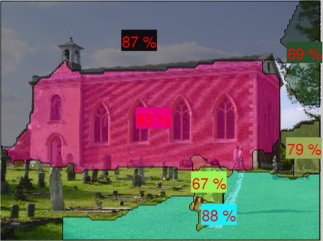
\includegraphics[width=0.15\textwidth]{figs/3_16_s_best_fragments.jpg}
%%    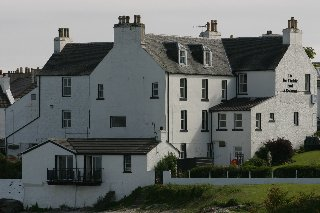
\includegraphics[width=0.15\textwidth]{figs/3_18_s.jpg}
%%   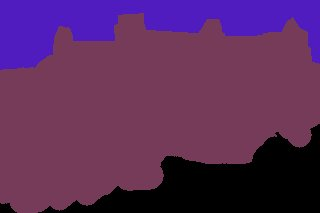
\includegraphics[width=0.15\textwidth]{figs/3_18_s_gt.jpg}
%%    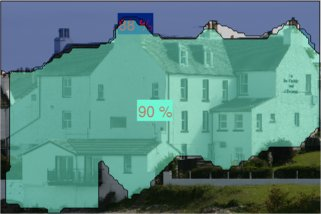
\includegraphics[width=0.15\textwidth]{figs/3_18_s_best_fragments.jpg}
%%       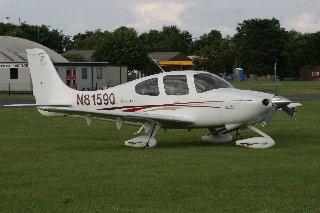
\includegraphics[width=0.15\textwidth]{figs/4_4_s.jpg}
%%   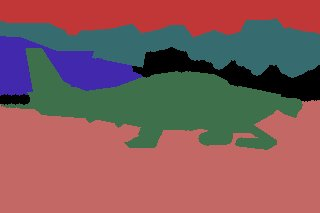
\includegraphics[width=0.15\textwidth]{figs/4_4_s_gt.jpg}
%%    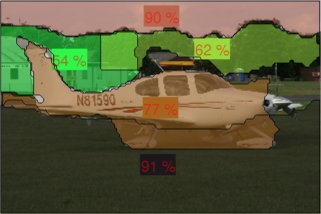
\includegraphics[width=0.15\textwidth]{figs/4_4_s_best_fragments.jpg}
%%       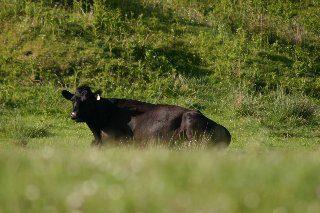
\includegraphics[width=0.15\textwidth]{figs/5_5_s.jpg}
%%   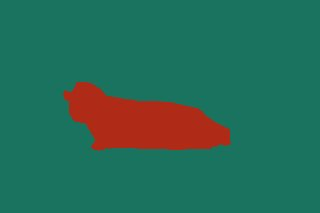
\includegraphics[width=0.15\textwidth]{figs/5_5_s_gt.jpg}
%%    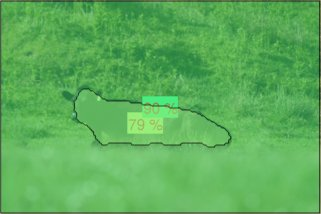
\includegraphics[width=0.15\textwidth]{figs/5_5_s_best_fragments.jpg}
%%     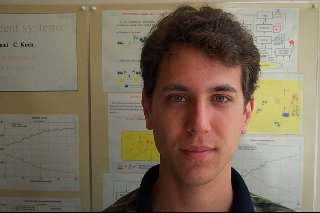
\includegraphics[width=0.15\textwidth]{figs/6_4_s.jpg}
%%   
\includegraphics[width=0.15\textwidth]{figs/6_4_s_gt.jpg}
%%    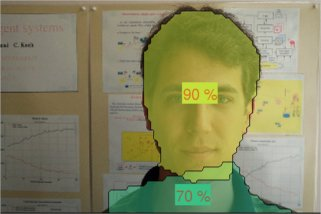
\includegraphics[width=0.15\textwidth]{figs/6_4_s_best_fragments.jpg}
%%     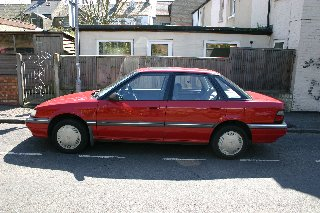
\includegraphics[width=0.15\textwidth]{figs/7_1_s.jpg}
%%   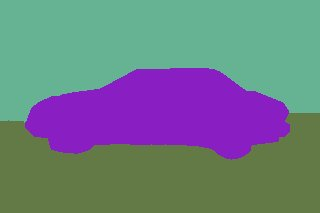
\includegraphics[width=0.15\textwidth]{figs/7_1_s_gt.jpg}
%%    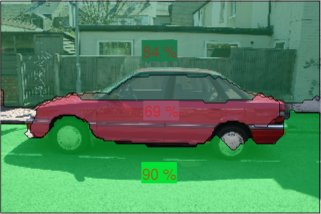
\includegraphics[width=0.15\textwidth]{figs/7_1_s_best_fragments.jpg}
%%       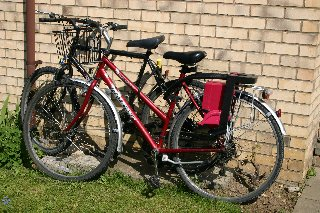
\includegraphics[width=0.15\textwidth]{figs/8_3_s.jpg}
%%   
\includegraphics[width=0.15\textwidth]{figs/8_3_s_gt.jpg}
%%    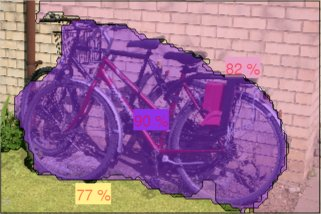
\includegraphics[width=0.15\textwidth]{figs/8_3_s_best_fragments.jpg}
%%   \begin{tabular}[b]{|c|c|c|}
%% \hline MSRC Dataset & Covering Score  \\
%% \hline Our Method  & {\bf 84.5}\\
%% \hline Carreira {\it etal}~\cite{Carreira:Sminchisescu:PAMI12}& 85  \\
%% %\hline Efros & XXX  \\
%% \hline Arbelaez {\it et al}~\cite{Arbelaez:etal:CVPR09} & 78.0  \\
%% \hline
%% \end{tabular}   
% 
\includegraphics[width=0.15\textwidth]{figs/11_10_s_gt.png}
%   
\includegraphics[width=0.15\textwidth]{figs/11_10_s_gt.png}
%    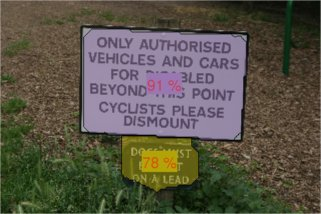
\includegraphics[width=0.15\textwidth]{figs/11_10_s_best_fragments.png}
% %  \includegraphics[width=0.15\textwidth]{figs/2007_000363.png}
% %  \includegraphics[width=0.15\textwidth]{figs/2007_000363_overlay.png}
% \includegraphics[width=0.15\textwidth]{figs/2008_000144.jpg}
%  \includegraphics[width=0.15\textwidth]{figs/2008_000144.png}
%  \includegraphics[width=0.15\textwidth]{figs/2008_000144_overlay.png}\\
% \includegraphics[width=0.15\textwidth]{figs/2009_002888.jpg}
%  \includegraphics[width=0.15\textwidth]{figs/2009_002888.png}
%  \includegraphics[width=0.15\textwidth]{figs/2009_002888_overlay.png}
% \includegraphics[width=0.15\textwidth]{figs/tisa.jpg} 
% \includegraphics[width=0.15\textwidth]{figs/tisa_jpg_gt.png}
%  \includegraphics[width=0.15\textwidth]{figs/tisa_overlay.png}\\
% %\vspace{-0.15cm}
   %%    \caption{\FigureFont The best object part hypotheses for MSRC\  examples and Covering Score.}
   %% \label{fig:MSRC}
%\vspace{-0.5cm}
%\end{figure}

% additional results in 

% The results presented in~\cite{Endres:Hoiem:ECCV10} probe  object recall
% for a minimum overlap requirement (50\%) on the best fragment covering the ground truth. We draw a comparison below.
%\hline Efros & XXX  \\
%\hline Arbelaez {\it et al}~\cite{Arbelaez:etal:CVPR09}
%BFS(F_{i}, {\cal \bar F}) = \max_{\bar F_{\bar i}\in{\cal \bar F}}J(F_i,\bar F_{\bar i})
  
% \smallskip
% {\small
% \begin{tabular}{|c|c|c|c|}\hline
% Segmentation Dataset & \# of images\ & Segmentation Mode & Objects  \\\hline
% Weizmann & 100 & Single Foreground Object & varied  \\\hline
% Berkeley BSDS 300 & 300 & Multiple Objects, Image Partition & varied \\\hline
% MSRC & 591 & Multiple Objects (\textasciitilde10 per image) & 23 Classes \\\hline
% ETHZ Shape Classes & 255 & Single or Multiple Objects & 5 Classes  \\\hline
% \end{tabular}


%\medskip




% \noindent
% \textbf{Evaluation:}
% Two sets $F_i$ and $\bar F_{\bar i}$, fragments  in our case, can be compared by measuring
% their intersection normalized by their union, namely, $J(A,B) = \frac{|F_i,\cap
% F_{\bar i}|}{|F_i,\cup F_{\bar i}|}.$ This has been referred to as \textit{overlap} in the object recognition literature but more generally is known as the  \textit{Jaccard Index}.  A group of fragments can be judged by whether there is a fragment that matches any given ground truth fragment and to what extent. The \textit{Best Fragment Score (\textbf{BFS})} for each ground truth segment is the maximum overlap measure over all computed fragments. 
% \begin{equation}
% %\vspace{-0.25cm}
% BFS(F_{i}, {\cal \bar F}) = \max_{\bar F_{\bar i}\in{\cal \bar F}}J(F_i,\bar F_{\bar i}).
% %\vspace{-0.125cm}
% \end{equation}
% The Mean BFS score (\textbf{MBFS})
% averages this measure over all ground truth segments and is the evaluation measure of choice in~\cite{malisiewicz:bmvc07,Carreira:Sminchisescu:PAMI12,Endres:Hoiem:ECCV10}.
% \noindent
%  We also need to compare two sets of segments,
% say computed fragments  ${\cal F}=\{F_1, F_2, \cdots, F_N\}$ 
% and  ground truth fragments  
%   ${\cal \bar F}=\{\bar F_1, \bar F_2, \cdots, \bar F_{\bar N}\}$. The
%   notion of \textit{covering}~\cite{Arbelaez:etal:CVPR09}  measures how well computed fragments ${\cal \bar F}$ cover ground
%   truth fragments in ${\cal  F,}$
% \begin{equation}
% %\vspace{-0.25cm}
% Covering({\cal F}, {\cal \bar F}) =\frac{\sum_{i=1}^N  BSF(F_{i}, {\cal \bar F})|\bar F_i| }{\sum_{i=1}^N |\bar F_i|} =\frac{\sum_{i=1}^N  |\bar F_i|\max_{\bar F_{\bar i}\in{\cal \bar F}}J(F_i,\bar F_{\bar i}) }{\sum_{i=1}^N |\bar F_i|}. 
% %\vspace{-0.0125cm}
% \end{equation} 
% \noindent
% \textbf{MSRC  Results:} Figure~\ref{fig:MSRC} shows the best fragment per
% annotated object for a selection from MSRC images. The Table below shows   that our algorithm is at part
% with thee state of the art in the segmentation task based on a comparison
% of the Covering measure and {\bf MBFS} over all objects across all categories. 
% \smallskip

% \begin{tabular}{|c|c|c|}
% \hline MSRC\ Datset & Covering Score  \\
% \hline Our Method  & 84.5\\
% \hline Carreira {\it et al}, PAMI12~\cite{Carreira:Sminchisescu:PAMI12}& 85  \\
% %\hline Efros & XXX  \\
% \hline Arbelaez {\it et al}~\cite{Arbelaez:etal:CVPR09} & 78.0  \\
% \hline
% \end{tabular}
% \begin{tabular}{|c|c|}
% \hline MSRC\ Dataset & Mean BFS score  \\
% \hline Our Method & 80 \\
% \hline Mean Shift & XX  \\
% \hline
% \end{tabular}




% %%%%%%%%%%%%%%%%                FIGURE          %%%%%%%%%%%%%%%%%%%%%
% \begin{figure}[!h]
%   %\vspace{-0.425cm}
% \includegraphics[width=0.32\linewidth]{figs/Mean_Shift_performance_versus_our_method.pdf}
% \includegraphics[width=0.32\linewidth]{figs/Ncut_performance_versus_our_method.pdf}
% \includegraphics[width=0.32\linewidth]{figs/FH_performance_versus_our_method.pdf}
% %\includegraphics[width=0.3\linewidth]{figs/pestov1.png}
%   %\vspace{-0.25cm}
%   \caption{\FigureFont Comparison against the Soup of Segments~approach \cite{malisiewicz:bmvc07} on the MSRC dataset for Mean Shift, Felzenszwalb and Huttenlocher, and NCuts. Notice that in many categories our fragments  are better, and even exceeding the upper-bound superpixel limit  for some, \eg, road. We expect that with the full implementation  
% the superpixel limit will be exceeded in additional categories.
% We thank the authors of~\cite{malisiewicz:bmvc07}
% for  this data. } 
% \label{fig:performance:category}
%   %\vspace{-0.4315cm}
% \end{figure}
%%%%%%%%%%%%%%%%%%%%%%%%%%%%%%%%%%%%%%%%%%%%%%%%%%

% \noindent
% \textbf{Berkeley Dataset} Figure~\ref{fig:BSDS:comparison} compares our results
% on the three BSDS examples explicitly shown in~\cite{Endres:Hoiem:ECCV10} with
% additional results in 
% Figure~\ref{fig:BSDS}.
% The results presented in~\cite{Endres:Hoiem:ECCV10} probe  object recall
% for a minimum overlap requirement (50\%) on the best fragment covering the ground truth. We draw a comparison below.


%%\vspace{-1cm}


% \begin{figure}[!h]
%   %\vspace{-0.13135cm}
% a\includegraphics[width=0.1\linewidth]{figs/41033.jpg}
% \includegraphics[width=0.1\linewidth]{figs/41033-hoiem-bf.png}
% \includegraphics[width=0.1\linewidth]{figs/41033_best_fragments.png}b
% \includegraphics[width=0.1\linewidth]{figs/8023.jpg}
% \includegraphics[width=0.1\linewidth]{figs/8023-hoiem-bf.png}
% \includegraphics[width=0.1\linewidth]{figs/8023_best_fragments.png}
% c\includegraphics[width=0.1\linewidth]{figs/38082.jpg}
% \includegraphics[width=0.1\linewidth]{figs/38082-hoiem-bf.png}
% \includegraphics[width=0.1\linewidth]{figs/38082_best_fragments.png}
% %\vspace{-0.5425cm}
% \caption{(a-c) Comparison to the  three BSDS examples shown in~\cite{Endres:Hoiem:ECCV10},
% each showing image, results from \cite{Endres:Hoiem:ECCV10} and ours showing
% a mix of results on this set. On average our results are slightly better.
%  }
%   \label{fig:BSDS:comparison}
%   %\vspace{-0.13525cm}
% \end{figure}

%% \begin{figure}[!ht]
%%  % %\vspace{-0.2752cm}
%% \centering
%% \includegraphics[width=0.155\textwidth]{figs/8049.jpg}
%%  \includegraphics[width=0.155\textwidth]{figs/8049_gt.jpg}
%% \includegraphics[width=0.155\textwidth]{figs/8049_best_fragments.jpg}
%% \includegraphics[width=0.155\textwidth]{figs/19021.jpg}
%%  \includegraphics[width=0.155\textwidth]{figs/19021_gt.jpg}
%% \includegraphics[width=0.155\textwidth]{figs/19021_best_fragments.jpg}
%% \includegraphics[width=0.155\textwidth]{figs/16052.jpg}
%%  \includegraphics[width=0.155\textwidth]{figs/16052_gt.jpg}
%%  \includegraphics[width=0.155\textwidth]{figs/16052_best_fragments.jpg}
%% \includegraphics[width=0.155\textwidth]{figs/69020.jpg}
%%  \includegraphics[width=0.155\textwidth]{figs/69020_gt.jpg}
%%  \includegraphics[width=0.155\textwidth]{figs/69020_best_fragments.jpg}
%%  \includegraphics[width=0.155\textwidth]{figs/100075.jpg}
%%  \includegraphics[width=0.155\textwidth]{figs/100075_gt.jpg}
%%  \includegraphics[width=0.155\textwidth]{figs/100075_best_fragments.jpg}
%%  % \includegraphics[width=0.15\textwidth]{figs/100075.jpg}
%%  % \includegraphics[width=0.15\textwidth]{figs/100075_gt.jpg}
%%  % \includegraphics[width=0.15\textwidth]{figs/100075_best_fragments.jpg}
%% \hspace{0.8cm} 
%% \begin{tabular}[!h]{|c|c|c|}
%%   \hline BSDS\ TestSet & Recall@50\% {\bf BFS}  \\
%%   \hline Our Method  & {\bf 87\%}\\
%%   \hline Endres {\em etal}~\cite{Endres:Hoiem:ECCV10} & 84\%  \\
%%   \hline  CPMC~\cite{Carreira:Sminchisescu:PAMI12} &  75\% \\
%%   \hline
%% \end{tabular}
%% % \includegraphics[width=0.15\textwidth]{figs/78019.jpg}
%%  % \includegraphics[width=0.15\textwidth]{figs/78019_gt.jpg}
%%  % \includegraphics[width=0.15\textwidth]{figs/78019_best_fragments.jpg}
%%  %  \includegraphics[width=0.15\textwidth]{figs/304034.jpg}
%%  %  \includegraphics[width=0.15\textwidth]{figs/304034_gt.jpg}
%%  %  \includegraphics[width=0.15\textwidth]{figs/304034_best_fragments.jpg}
%%  % \includegraphics[width=0.15\textwidth]{figs/108073.jpg}
%%  % \includegraphics[width=0.15\textwidth]{figs/108073_gt.jpg}
%%  % \includegraphics[width=0.15\textwidth]{figs/108073_best_fragments.jpg}
%% % \includegraphics[width=0.15\textwidth]{figs/23025.jpg}
%% %  \includegraphics[width=0.15\textwidth]{figs/23025_gt.png}
%% % \includegraphics[width=0.15\textwidth]{figs/23025_best_fragments.png}
%% % %\vspace{-0.15cm}
%%       \caption{\FigureFont The best object part hypotheses for examples from the Berkeley dataset.}
%%    \label{fig:BSDS}
%% %\vspace{-0.65cm}
%% \end{figure}

%% When evaluating any segmentation algorithm, it is also important to asses the number of segments produced. Ideally one would like as few as possible fragments, while still maintaining segmentation quality. Our current scheme for reducing the number of fragments is very simple at this stage: in a visitation schedule of fragments we remove all fragments whose overlap with retained fragments exceeds a threshold. For example, for the BSDS300 Test dataset the object recall at the pascal criterion is 86\% with 8600 fragments. More complex clustering algorithms together with a ranking procedure (as used in~\cite{Carreira:Sminchisescu:PAMI12,Endres:Hoiem:ECCV10}) should reduce this at least another order of magnitude or more, although we are now exploring this. The fragments produced by our approach match or slightly exceed the state of the art in segmenting figure from ground, even though the focus of our approach is not really figure ground segregation but rather generating object part hypotheses. The proper evaluation of this aspect motivates the introduction of a new measure.
% 
% \begin{figure}[!h]
%   \includegraphics[width=0.5\linewidth]{figs/02_27_12_Our_Method_vs_Hoiem.pdf}
%   \caption{a) Object Recall vs Jacard Index for the BDS shows a comparison
% with the work of HOIEM.}
%   \label{fig:bsds_object_recall}
% \end{figure}

%%\vspace{-0.5cm}
%% \textbf{Evaluation of Fragmentation:} The obvious distinction between evaluation of Figure-Ground segregation algorithms and those that are expected to generate object parts is that in the latter the fragments are not necessarily expected to cover the entire object with a single fragment. The expectation from a good ``fragmentation algorithm'' is that each object would be covered with as few fragments as possible, and as accurately as possible. First a fragment ${\bar F}_{\bar i}$, should participate in describing an object $ {F}_{i}$ only if it accurately describes a portion of it,\textit{ i.e.,} participating fragments are expected
%% to have  high precision, $\frac {|F_i\cap {\bar F}_{\bar i}|} {|{\bar F}_{\bar i}|} > \tau_p$ 
%% %\begin{equation}
%% %  %\vspace{-0.255cm}
%%  %    ,
%%         % %\vspace{-0.105cm}
%% %\end{equation}
%% where $\tau_p$ is a constant close to 1, \emph{e.g}, $\tau_p=0.95.$
%% Second a set of high precision fragments $\{{\bar F}_{{\bar i}_1},{\bar F}_{{\bar i}_2},...,{\bar F}_{{\bar i}_K}\}$ can accurately describe an object if their union has high percent object recall,$\frac {| {F}_{i}\cap(\bigcup_{k=1}^{K}{\bar F}_{{\bar i}_{k}})|} {|{F}_{i}|}$. Third, since any object can be covered well with a very large number of
%% fine-grained fragments, good coverage needs to be counterbalanced with
%% the number of fragments used to describe the object. Thus, our approach to the evaluation of fragments trades off cumulative percent object recall
%% versus the number of fragments used to describe the object, as measured on a pool of high
%% precision fragments. Since the selection of which subset of fragments should
%% be used to explain the object is combinatorially large we take a greedy approach to it: The best fragment in the pool of high precision
%% fragments is selected as the first fragment, the set of object pixels explained
%% by this fragment is removed from contributing to future recall values and the remaining part of the object is probed
%% for coverage by the remaining high precision fragments. In other words, given that $l$
%% fragments have been selected, the $l+1^{th}$ fragment is selected by
%% \begin{equation*}
%% \begin{split}
%% %%\vspace{-0.325cm}
%% \min_{j\not \in\{i_{1},i_2,\cdots,i_l\} }\frac {| [{F}_{i}-(\bigcup_{k=1}^{l}{\bar F}_{{\bar i}_{k}})]\cap F_{j}|} {|F_{i}-(\bigcup_{k=1}^{l}{\bar F}_{{\bar i}_{k}})|} = \\
%% \min_{j\not \in\{i_{1},i_2,\cdots,i_l\}}  {| {F}_{i}\cap {\bar F}_{\bar j}-(\bigcup_{k=1}^{l}{\bar F}_{{\bar i}_{k}})\cap {\bar F}_{\bar j}|}
%% \end{split} 
%% \end{equation*} This procedure is illustrated in Figure~\ref{fig:fragment:evaluation:example}


% To evaluate fragmentation versus segmentation experiments were based on the
% database used in~\cite{Endres:Hoiem:ECCV10}, which are annotations of images from the BSDS300 Test set. This dataset can be  found at \url{http://vision.cs.uiuc.edu/proposals}.  For each ground truth object, the {\it percent-object recall},Equation~\ref{eq:percent}, is examined as a function of the number of fragments, both for our method and for segments from~\cite{Carreira:Sminchisescu:PAMI12} which we obtained from the code kindly shared by them: \url{http://sminchisescu.ins.uni-bonn.de/code/cpmc}.
%% Figure~\ref{fig:cpmc_vs_ours1} shows the fragmentation score  averaged over the entire BSDS300 Test dataset. 
%% Observe that the best high precision fragment of~\cite{Carreira:Sminchisescu:PAMI12} covers slightly more of the object than our best high precision fragment does. However, as more fragments are included, our fragments outperform those of~\cite{Carreira:Sminchisescu:PAMI12}.  This is somewhat expected as the stated goal of~\cite{Carreira:Sminchisescu:PAMI12} is to provide figure ground segmentation through many tries, while our stated goal is to produce object part fragments.

% Alternatively, we can fix the number of fragments $K$ and observe the
% trade-off between object recall and minimum fragment precision $\tau_p$.
% 


%% \begin{figure}[!t]
%% %\vspace{-0.2325cm}
%% \footnotesize{\textit{a}} \includegraphics[height=0.09412\linewidth]{figs/160068_top_1_fragments.jpg}
%% \footnotesize{\textit{b}} \includegraphics[height=0.09412\linewidth]{figs/160068_top_2_fragments.jpg}
%% \footnotesize{\textit{c}} \includegraphics[height=0.09412\linewidth]{figs/160068_top_3_fragments.jpg}
%% \footnotesize{\textit{d}} \includegraphics[height=0.09412\linewidth]{figs/160068_top_4_fragments.jpg}
%% \footnotesize{\textit{e}} \includegraphics[height=0.09412\linewidth]{figs/160068_top_20_fragments_montage.jpg}
%% \footnotesize{\textit{f}} \includegraphics[height=0.09412\linewidth]{figs/160068_object_recall_vs_fragments.pdf}
%% % \\\footnotesize{\textit{a}} \includegraphics[height=0.09412\linewidth]{figs/37073_top_1_fragments.jpg}
%% % \footnotesize{\textit{b}} \includegraphics[height=0.09412\linewidth]{figs/37073_top_2_fragments.jpg}
%% % \footnotesize{\textit{c}} \includegraphics[height=0.09412\linewidth]{figs/37073_top_5_fragments.jpg}
%% % \footnotesize{\textit{d}} \includegraphics[height=0.09412\linewidth]{figs/37073_top_6_fragments.jpg}
%% % \footnotesize{\textit{e}} \includegraphics[height=0.09412\linewidth]{figs/37073_top_20_fragments_montage.png}
%% % \footnotesize{\textit{f}} \includegraphics[height=0.09412\linewidth]{figs/37073_object_recall_vs_fragments.pdf}
%% %\vspace{-0.2cm}
%% \caption{An illustration of evaluating the value of fragments to describe objects from a sample of BSDS.}
%%   \label{fig:fragment:evaluation:example}
%%   %\vspace{-0.325cm}
%% \end{figure}

%% %\vspace{-0.5cm}

%% \begin{figure}[h!]
%%   \centering
%%   \includegraphics[width=0.7\linewidth]{figs/03_12_12_fragmentation_score_full_bsdtest.pdf}  
%%   \caption{Average Fragmentation Measure at $\tau_p=0.90,0.95$ for Test Set of BSDS300}
%%   \label{fig:cpmc_vs_ours1}

%% \end{figure}

%\vspace{-1cm}

% \begin{figure}[!h]
% (a) %\includegraphics[width=0.5\linewidth]{figs/17_14_s_best_fragments.png}
% (b) % \includegraphics[width=0.5\linewidth]{figs/02_28_12_per_category_recall_vs_jacard.pdf}
% \caption{The plot of object recall vs the number of fragments for several
% minimum precision values evaluated  fragmentation  on MSRC
% and BSDS.}
%   \label{fig:fragment:evaluation}
%   %\vspace{-0.325cm}
% \end{figure}
% 
% \noindent\textbf{Evaluation of Fragmentation for Recognition:}
% One way to measure the quality of a fragmentation algorithm is to measure
% the recognizability of the fragments generated. We use the approached used
% in~\cite{Gu:Malik:CVPR09:Region} to evaluate the fragments generated here.
% The Table below compares
% that object detection performance on the ETHZ Shape Classes Dataset~\cite{Ferrari:Tuytelaars:VanGool:ECCV06}. The two numbers in each cell of the table correspond to the Detection Rates at FPPI (false positives per image) 0.3 and 0.4, respectively.

% \begin{tabular}{|c||c|c|c|c|c||c|}
% \hline
% Category                             & applelogo & bottle & giraffe & mug & swan & Average\\
%  \hline
%  Ferrari  \cite{Ferrari:Fevrier:Jurie:Schmid:PAMI08} &          50.0/60.0 &  92.9/92.9 & 49.0/51.1 & 67.8/77.4 & 47.1/52.4 & 61.4/66.8\\
%  \hline
% % Fritz CVPR08~\cite{Fritz:Schiele:CVPR08} & -/83.2 & -/83.2 & -/58.6 & -/83.6 & -/75.4 & -/76.8\\
% % \hline
% % Felz. CVPR08~\cite{Felzenszwalb:etal:CVPR08} code & 95.0/95.0 & 1/1 & 72.9/72.9 & 83.9/83.9 & 58.8/64.7 & 82.1/83.3\\
% % \hline
% % Zhu ECCV08~\cite{Zhu:etal:ECCV08},hand-drawn  & 80.0/80.0  &  92.9/92.9 & 68.1/68.1  & 64.5/74.2  & 82.4/82.4  & 77.6/79.5  \\
% % \hline
% % Ravishankar ECCV08~\cite{Ravishankar:etal:ECCV08},hand-drawn & 95.5/97.7 & 90.9/92.7 & 91.2/93.4 & 93.7/95.3 & 93.9/96.9 & 93.0/95.2 \\
% % \hline
% % Gu CVPR09~\cite{Gu:etal:CVPR09} &  90.6/- & 94.8/- & 79.8/- & 83.2/- & 86.8/- &87.1/-\\
% % \hline
% % Maji CVPR09~\cite{Gu:etal:CVPR09} &  95.0/95.0 & 92.9/96.4 & 89.6/89.6 & 93.6/96.7 & 88.2/88.2 &91.9/93.2\\
% % \hline
% % Lu ICCV09~\cite{Lu:etal:ICCV09},hand-drawn & 90.0/90.9 & 79.2/79.2 & 73.4/77.0 & 81.3/83.3 & 93.8/93.8 & 83.6/85.1 \\
% % \hline
% % Ommer ICCV09~\cite{Ommer:Malik:ICCV09} & 95.0/95.0 & 89.3/89.3 & 70.5/75.4 &  87.3/90.3 & 94.1/94.1 & 87.2/88.8\\
% % \hline
% % Srinivasan CVPR10~\cite{Srinivasan:etal:CVPR10} & 95.0/95.0  & 1/1 & 87.2/89.6  & 93.6/93.6  & 1/1  & 95.2/95.6  \\
% % \hline
% % Liu CVPR10~\cite{Liu:etal:CVPR10} (PR/FPPI) &  &  &  &  &  &  \\
% % \hline
% % Riemenschneider ECCV10~\cite{Riemenschneider:etal:ECCV10} & 93.3/93.3  & 97.0/97.0  & 79.2/81.9  & 84.6/86.3  & 92.6/92.6  & 89.3/90.5  \\
% % \hline
% % Wang ECCV10~\cite{Wang:etal:ECCV10} (PR/FPPI) &  &  &  &  &  &  \\
% % \hline
% % Yang ACCV10~\cite{Yang:Latecki:ACCV10} & 80.0/80.0 & 92.9/95.9 & 76.92/79.21 & 83.3/84.85 & 90.9/94.1 & 84.8/86.79 \\
% % \hline
% % Ferrari IJCV10 (full system)~\cite{Ferrari:etal:IJCV10} & 77.7/83.2 & 79.8/81.6 & 39.9/44.5 &75.1/80.0 & 63.2/70.5 & 67.2/72.0\\
% % \hline
% % Ma CVPR11~\cite{Ma:Latecki:CVPR11} & 92.0/92.0 &  97.9/97.9 &  85.4/85.4 & 87.5/87.5 &  1/1 &  92.6/92.6\\
% % \hline
% Trinh ~\cite{Trinh:Kimia:IJCV11} & 91.7/91.7&  96.8/96.8 &  89.8/91.8 & 70.7/80.5 &  94.1/100 &  88.6/92.1\\
% \hline
% Gu \cite{Gu:Malik:CVPR09:Region} & 90.5/90.5&  96.7/96.7 &  79.6/79.6 & 81.8/81.8 &  87.5/87.5 &  -/-\\
% % \hline
% % Our Method & 54.17/58.33&  60.0/60.0 &  75.56/75.56 & 75.68/78.38 &  76.47/82.35 &  -/-\\
% \hline
% Our Method & 70.83/79.17&  60.0/66.7 &  64.4/64.4 & 75.68/75.68 &  41.2/64.71 &  -/-\\
% \hline
% \end{tabular}



% 
% \begin{figure}[!h]
% \includegraphics[width=0.45\linewidth]{figs/02_25_12_pr_vs_recall_overlay_F_measure.pdf}
% \begin{tabular}[b]{|c|c|}
%  \hline Weizmann Seg.Dataset & F-Meas. \\
% \hline Carreira etal, PAMI12~\cite{Carreira:Sminchisescu:PAMI12}
% & 93 \\ 
% \hline Our Method & 89  \\
% \hline Bagon etal ECCV08~\cite{Bagon:etal:ECCV08} & 87  \\
% \hline Alpert etal CVPR07~\cite{Alpert:etal:CVPR07} & 86\\
% \hline Galun etal ICCV03~\cite{Galun:etal:ICCV03}&83\\
% \hline
% \end{tabular}
%      \caption{\FigureFont Distribution of Fragments in the PR domain for
%       the Weizmann Dataset.}
%    \label{fig:BT1}
%\end{figure}
% \footnote{It should
% be noted that when fragments are used for recognition or multiview matching, the evaluation can be
% relaxed so that the entire object may not have to be covered, but rather
% the fragments
% are expected to be 
%  recognizable or repeatable, respectively.} 


\begin{figure*}[!ht]
  \centering
{\footnotesize\textit{\textcolor{white}{a)}}}\includegraphics[width=0.31\linewidth]{figs/94079_00.png}
{\footnotesize\textit{\textcolor{white}{a)}}}\includegraphics[width=0.31\linewidth]{figs/94079_gt.png}
{\footnotesize\textit{\textcolor{white}{a)}}}\includegraphics[width=0.31\linewidth]{figs/94079_mvf.png}

{\footnotesize\textit{\textcolor{white}{a)}}}\includegraphics[width=0.31\linewidth]{figs/370036_00.png}
{\footnotesize\textit{\textcolor{white}{a)}}}\includegraphics[width=0.31\linewidth]{figs/370036_gt.png}
{\footnotesize\textit{\textcolor{white}{a)}}}\includegraphics[width=0.31\linewidth]{figs/370036_mvf.png}

{\footnotesize\textit{\textcolor{white}{a)}}}\includegraphics[width=0.31\linewidth]{figs/323016_00.png}
{\footnotesize\textit{\textcolor{white}{a)}}}\includegraphics[width=0.31\linewidth]{figs/323016_gt.png}
{\footnotesize\textit{\textcolor{white}{a)}}}\includegraphics[width=0.31\linewidth]{figs/323016_mvf.png}


{\footnotesize\textit{\textcolor{white}{a)}}}\includegraphics[width=0.31\linewidth]{figs/253027_00.png}
{\footnotesize\textit{\textcolor{white}{a)}}}\includegraphics[width=0.31\linewidth]{figs/253027_gt.png}
{\footnotesize\textit{\textcolor{white}{a)}}}\includegraphics[width=0.31\linewidth]{figs/253027_mvf.png}

{\footnotesize\textit{\textcolor{white}{a)}}}\includegraphics[width=0.31\linewidth]{figs/38092_00.png}
{\footnotesize\textit{\textcolor{white}{a)}}}\includegraphics[width=0.31\linewidth]{figs/38092_gt.png}
{\footnotesize\textit{\textcolor{white}{a)}}}\includegraphics[width=0.31\linewidth]{figs/38092_mvf.png}

{\footnotesize\textit{\textcolor{black}{a)}}}\includegraphics[width=0.31\linewidth]{figs/157055_00.png}
{\footnotesize\textit{\textcolor{black}{b)}}}\includegraphics[width=0.31\linewidth]{figs/157055_gt.png}
{\footnotesize\textit{\textcolor{black}{c)}}}\includegraphics[width=0.31\linewidth]{figs/157055_mvf.png}

\caption{a) Images from BSDS300. b) Ground-Truth Annotations by~\cite{Endres:Hoiem:PAMI14} c) Our best proposals according to Jaccard Index overlaid over the ground-truth objects. }
 \label{fig:bsds_examples}
%\vspace{-0.751cm}
 \end{figure*}



\begin{figure*}[!ht]
  \centering
{\footnotesize\textit{\textcolor{white}{a)}}}\includegraphics[width=0.31\linewidth]{figs/3_5_s_00.png}
{\footnotesize\textit{\textcolor{white}{a)}}}\includegraphics[width=0.31\linewidth]{figs/3_5_s_gt.png}
{\footnotesize\textit{\textcolor{white}{a)}}}\includegraphics[width=0.31\linewidth]{figs/3_5_s_mvf.png}

%% {\footnotesize\textit{\textcolor{white}{a)}}}\includegraphics[width=0.31\linewidth]{figs/3_6_s_00.png}
%% {\footnotesize\textit{\textcolor{white}{a)}}}\includegraphics[width=0.31\linewidth]{figs/3_6_s_gt.png}
%% {\footnotesize\textit{\textcolor{white}{a)}}}\includegraphics[width=0.31\linewidth]{figs/3_6_s_mvf.png}

%% {\footnotesize\textit{\textcolor{white}{a)}}}\includegraphics[width=0.31\linewidth]{figs/3_22_s_00.png}
%% {\footnotesize\textit{\textcolor{white}{a)}}}\includegraphics[width=0.31\linewidth]{figs/3_22_s_gt.png}
%% {\footnotesize\textit{\textcolor{white}{a)}}}\includegraphics[width=0.31\linewidth]{figs/3_22_s_mvf.png}

{\footnotesize\textit{\textcolor{white}{a)}}}\includegraphics[width=0.31\linewidth]{figs/10_7_s_00.png}
{\footnotesize\textit{\textcolor{white}{a)}}}\includegraphics[width=0.31\linewidth]{figs/10_7_s_gt.png}
{\footnotesize\textit{\textcolor{white}{a)}}}\includegraphics[width=0.31\linewidth]{figs/10_7_s_mvf.png}

{\footnotesize\textit{\textcolor{white}{a)}}}\includegraphics[width=0.31\linewidth]{figs/1_18_s_00.png}
{\footnotesize\textit{\textcolor{white}{a)}}}\includegraphics[width=0.31\linewidth]{figs/1_18_s_gt.png}
{\footnotesize\textit{\textcolor{white}{a)}}}\includegraphics[width=0.31\linewidth]{figs/1_18_s_mvf.png}

%% {\footnotesize\textit{\textcolor{white}{a)}}}\includegraphics[width=0.31\linewidth]{figs/6_14_s_00.png}
%% {\footnotesize\textit{\textcolor{white}{a)}}}\includegraphics[width=0.31\linewidth]{figs/6_14_s_gt.png}
%% {\footnotesize\textit{\textcolor{white}{a)}}}\includegraphics[width=0.31\linewidth]{figs/6_14_s_mvf.png}


%% {\footnotesize\textit{\textcolor{white}{a)}}}\includegraphics[width=0.31\linewidth]{figs/6_14_s_00.png}
%% {\footnotesize\textit{\textcolor{white}{a)}}}\includegraphics[width=0.31\linewidth]{figs/6_14_s_gt.png}
%% {\footnotesize\textit{\textcolor{white}{a)}}}\includegraphics[width=0.31\linewidth]{figs/6_14_s_mvf.png}

{\footnotesize\textit{\textcolor{white}{a)}}}\includegraphics[width=0.31\linewidth]{figs/16_1_s_00.png}
{\footnotesize\textit{\textcolor{white}{a)}}}\includegraphics[width=0.31\linewidth]{figs/16_1_s_gt.png}
{\footnotesize\textit{\textcolor{white}{a)}}}\includegraphics[width=0.31\linewidth]{figs/16_1_s_mvf.png}


%% {\footnotesize\textit{\textcolor{white}{a)}}}\includegraphics[width=0.31\linewidth]{figs/16_20_s_00.png}
%% {\footnotesize\textit{\textcolor{white}{a)}}}\includegraphics[width=0.31\linewidth]{figs/16_20_s_gt.png}
%% {\footnotesize\textit{\textcolor{white}{a)}}}\includegraphics[width=0.31\linewidth]{figs/16_20_s_mvf.png}

{\footnotesize\textit{\textcolor{white}{a)}}}\includegraphics[width=0.31\linewidth]{figs/18_25_s_00.png}
{\footnotesize\textit{\textcolor{white}{a)}}}\includegraphics[width=0.31\linewidth]{figs/18_25_s_gt.png}
{\footnotesize\textit{\textcolor{white}{a)}}}\includegraphics[width=0.31\linewidth]{figs/18_25_s_mvf.png}

{\footnotesize\textit{\textcolor{black}{a)}}}\includegraphics[width=0.31\linewidth]{figs/10_12_s_00.png}
{\footnotesize\textit{\textcolor{black}{b)}}}\includegraphics[width=0.31\linewidth]{figs/10_12_s_gt.png}
{\footnotesize\textit{\textcolor{black}{c)}}}\includegraphics[width=0.31\linewidth]{figs/10_12_s_mvf.png}


\caption{a) Images from MSRC. b) Ground-Truth Annotations by Soup of Segments~\cite{malisiewicz:bmvc07} c) Our best proposals according to Jaccard Index overlaid over the ground-truth objects. }
 \label{fig:msrc_examples}
%\vspace{-0.751cm}
 \end{figure*}

\begin{figure*}[!ht]
  \centering
{\footnotesize\textit{\textcolor{white}{a)}}}\includegraphics[width=0.31\linewidth]{figs/003020_00.png}
{\footnotesize\textit{\textcolor{white}{a)}}}\includegraphics[width=0.31\linewidth]{figs/003020.png}
{\footnotesize\textit{\textcolor{white}{a)}}}\includegraphics[width=0.31\linewidth]{figs/003020_mvf.png}

{\footnotesize\textit{\textcolor{white}{a)}}}\includegraphics[width=0.31\linewidth]{figs/009817_00.png}
{\footnotesize\textit{\textcolor{white}{a)}}}\includegraphics[width=0.31\linewidth]{figs/009817.png}
{\footnotesize\textit{\textcolor{white}{a)}}}\includegraphics[width=0.31\linewidth]{figs/009817_mvf.png}

%% {\footnotesize\textit{\textcolor{white}{a)}}}\includegraphics[width=0.31\linewidth]{figs/005759_00.png}
%% {\footnotesize\textit{\textcolor{white}{a)}}}\includegraphics[width=0.31\linewidth]{figs/005759.png}
%% {\footnotesize\textit{\textcolor{white}{a)}}}\includegraphics[width=0.31\linewidth]{figs/005759_mvf.png}

{\footnotesize\textit{\textcolor{white}{a)}}}\includegraphics[width=0.31\linewidth]{figs/009346_00.png}
{\footnotesize\textit{\textcolor{white}{a)}}}\includegraphics[width=0.31\linewidth]{figs/009346.png}
{\footnotesize\textit{\textcolor{white}{a)}}}\includegraphics[width=0.31\linewidth]{figs/009346_mvf.png}

%% {\footnotesize\textit{\textcolor{white}{a)}}}\includegraphics[width=0.31\linewidth]{figs/008256_00.png}
%% {\footnotesize\textit{\textcolor{white}{a)}}}\includegraphics[width=0.31\linewidth]{figs/008256.png}
%% {\footnotesize\textit{\textcolor{white}{a)}}}\includegraphics[width=0.31\linewidth]{figs/008256_mvf.png}

{\footnotesize\textit{\textcolor{white}{a)}}}\includegraphics[width=0.31\linewidth]{figs/008708_00.png}
{\footnotesize\textit{\textcolor{white}{a)}}}\includegraphics[width=0.31\linewidth]{figs/008708.png}
{\footnotesize\textit{\textcolor{white}{a)}}}\includegraphics[width=0.31\linewidth]{figs/008708_mvf.png}

{\footnotesize\textit{\textcolor{white}{a)}}}\includegraphics[width=0.31\linewidth]{figs/009435_00.png}
{\footnotesize\textit{\textcolor{white}{a)}}}\includegraphics[width=0.31\linewidth]{figs/009435.png}
{\footnotesize\textit{\textcolor{white}{a)}}}\includegraphics[width=0.31\linewidth]{figs/009435_mvf.png}

\caption{a) Images from PASCAL VOC 2007 challenge. b) Ground-Truth Annotations from the dataset. c) Our best proposals according to Jaccard Index overlaid over the ground-truth objects. }
 \label{fig:voc_examples}
%\vspace{-0.751cm}
 \end{figure*}

\clearpage
\subsection{Evaluation of Part Proposals}

We evaluate the ability of our approach to generate meaningful parts in two ways: \emph{(i)} performance against an annotated database of parts and \emph{(ii)} measuring the ability to recover the whole object with multiple fragments, which we refer to as ``Fragmentation'' measure. 

\begin{figure*}[p]
\begin{center}
\scriptsize
\raisebox{-0.5\height}{{\footnotesize\textit{\textcolor{black}{a}}}}
\begin{tabular}{ |l|P{1.1cm}|P{1.1cm}|P{1.1cm}|P{1.1cm}|P{1.1cm}|P{1.27cm}| }
\hline
\multicolumn{7}{|c|}{Part Dataset}\\
\hline
Method & Mean Jaccard Parts & Mean Jaccard Legs & Mean Jaccard Body & Mean Jaccard Head & Mean Jaccard Tail & Mean Number Regions\\
\hline
\rowcolor{cyan} {\bf Our Method} & {\bf  61.80} & {\bf  59.60} & {\bf  72.75} & {\bf  69.46} & {\bf  54.13} & {\bf 5649.53} \\
\hline
MCG~\cite{Arbelaez:etal:CVPR14} &  59.21 &  50.73 &  71.10 &  66.93 &  52.88 & 3879.74\\
\hline
GOP~\cite{Krahenbuhl:Koltun:ECCV14} &  55.94 &  47.13 &  68.26 &  65.18 &  46.62 & 702.79\\
\hline
LPO~\cite{Krahenbuhl:Koltun:CVPR15} &  55.41 &  44.35 &  70.03 &  67.20 &  45.23 & 563.13\\
\hline
gPb-owt-ucm~\cite{Arbelaez:etal:PAMI11} &  55.39 &  51.53 &  65.02 &  54.32 &  53.05 & 2850.48\\
\hline
Rantalankila~\cite{Rantalankila:etal:CVPR14} &  53.95 &  44.09 &  67.27 &  63.43 &  46.60 & 1548.45\\
\hline
CIP~\cite{Endres:Hoiem:PAMI14} &  51.94 &  40.84 &  68.68 &  61.81 &  41.42 & 1261.85\\
\hline
Rigor~\cite{Humayun:etal:CVPR14} &  51.22 &  38.60 &  69.04 &  63.52 &  39.57 & 1109.92\\
\hline
CPMC~\cite{Carreira:Sminchisescu:PAMI12} &  47.78 &  34.09 &  67.67 &  61.02 &  34.12 & 576.71\\
\hline
Shape Sharing~\cite{Kim:Grauman:ECCV12} &  47.59 &  31.69 &  71.34 &  61.83 &  32.45 & 1142.80\\
\hline
\end{tabular}
{\footnotesize\textit{\textcolor{black}{b}}}\includegraphics[width=0.34\textwidth]{figs/part_recall.pdf}
{\footnotesize\textit{\textcolor{black}{c}}}\includegraphics[width=0.34\textwidth]{figs/leg_recall.pdf}
{\footnotesize\textit{\textcolor{black}{d}}}\includegraphics[width=0.34\textwidth]{figs/body_recall.pdf}
{\footnotesize\textit{\textcolor{black}{e}}}\includegraphics[width=0.34\textwidth]{figs/head_recall.pdf}
{\footnotesize\textit{\textcolor{black}{f}}}\includegraphics[width=0.34\textwidth]{figs/tail_recall.pdf}

\end{center}
\caption{ We evaluate our approach on Quadrapeds~\cite{Wang:etal:ICCV15}. (a) The table captures our various metrics. (b) Part recall for all parts. (c) Leg part recall. (d) Body part recall. (e) Head part recall. (f) Tail part recall. Observe that our approach achieves state of the art results across the various metrics and in terms of the behavior of our part-recall curves. }
\label{fig:part_results} 
\end{figure*}

%% In the case, of full-objects there is much more consistency across human subjects in terms of ground-truth labeling. In the case of parts it is not directly obvious how parts should be annotated and furthermore there is much more disagreement across human subjects.

\noindent\\
{\bf Evaluation of Annotated Parts: } Here we perform the same analysis as with full object proposals, Figure~\ref{fig:part_results}. First, observe that the performance of all algorithms across the board is much lower in the case of part proposals than in the case of full object proposals. Second, observe that the performance of our approach which was second best, just slightly below the performance of MCG~\cite{Arbelaez:etal:CVPR14}, now takes the lead across all metrics of comparisons. This lead is consistent across all parts, although it ranges from $\pm 9\%$ for legs to  $\pm 3\%$ for tails, Figure~\ref{fig:part_results}, as compared to the second best method which is MCG. Qualitative examples are shown in Figure~\ref{fig:part_examples}.

 %% This can be observed in Figure~\ref{fig:part_results}\textcolor{red}{(a)} where  Figure~\ref{fig:part_results}\textcolor{red}{(a)} tabulates the jaccard index over all parts and also individually. For example, we observe that across all parts we maintain a mean average Jaccard Index of roughly $62\%$ but if we look specifically at legs we observe that our average jaccard index of $60\%$ is roughly $10\%$ percent higher than the next best method. If we quantify our performance in terms of an object recall curve, legs in Figure~\ref{fig:part_results}\textcolor{red}{(c)}, body in Figure~\ref{fig:part_results}\textcolor{red}{(d)}, head in  Figure~\ref{fig:part_results}\textcolor{red}{(e)}, tail in Figure~\ref{fig:part_results}\textcolor{red}{(f)}, we observe that our most prominent advantage is in legs, body, and head, while we struggle with tails. Again, similar to the full-object proposal evaluation the next best competing method is MCG. Overall we observe that our performance across the board is the highest irrespective of metric. Finally, similar to the full-object proposal evaluation we show qualitative results in Figure~\ref{fig:part_examples}. 






\begin{figure*}[!ht]
  \centering
{\footnotesize\textit{\textcolor{white}{a)}}}\includegraphics[width=0.30\linewidth]{figs/2009_002097_00.jpg}
{\footnotesize\textit{\textcolor{white}{a)}}}\includegraphics[width=0.30\linewidth]{figs/2009_002097_part_mask.png}
{\footnotesize\textit{\textcolor{white}{a)}}}\includegraphics[width=0.30\linewidth]{figs/2009_002097_mvf.png}

{\footnotesize\textit{\textcolor{white}{a)}}}\includegraphics[width=0.30\linewidth]{figs/2008_002859_00.jpg}
{\footnotesize\textit{\textcolor{white}{a)}}}\includegraphics[width=0.30\linewidth]{figs/2008_002859_part_mask.png}
{\footnotesize\textit{\textcolor{white}{a)}}}\includegraphics[width=0.30\linewidth]{figs/2008_002859_mvf.png}

{\footnotesize\textit{\textcolor{white}{a)}}}\includegraphics[width=0.30\linewidth]{figs/2008_003379_00.jpg}
{\footnotesize\textit{\textcolor{white}{a)}}}\includegraphics[width=0.30\linewidth]{figs/2008_003379_part_mask.png}
{\footnotesize\textit{\textcolor{white}{a)}}}\includegraphics[width=0.30\linewidth]{figs/2008_003379_mvf.png}

{\footnotesize\textit{\textcolor{white}{a)}}}\includegraphics[width=0.30\linewidth]{figs/2008_007378_00.jpg}
{\footnotesize\textit{\textcolor{white}{a)}}}\includegraphics[width=0.30\linewidth]{figs/2008_007378_part_mask.png}
{\footnotesize\textit{\textcolor{white}{a)}}}\includegraphics[width=0.30\linewidth]{figs/2008_007378_mvf.png}

{\footnotesize\textit{\textcolor{white}{a)}}}\includegraphics[width=0.30\linewidth]{figs/2009_000931_00.jpg}
{\footnotesize\textit{\textcolor{white}{a)}}}\includegraphics[width=0.30\linewidth]{figs/2009_000931_part_mask.png}
{\footnotesize\textit{\textcolor{white}{a)}}}\includegraphics[width=0.30\linewidth]{figs/2009_000931_mvf.png}

%% {\footnotesize\textit{\textcolor{white}{a)}}}\includegraphics[width=0.30\linewidth]{figs/2008_002859_00.jpg}
%% {\footnotesize\textit{\textcolor{white}{a)}}}\includegraphics[width=0.30\linewidth]{figs/2008_002859_part_mask.png}
%% {\footnotesize\textit{\textcolor{white}{a)}}}\includegraphics[width=0.30\linewidth]{figs/insert.png}

%% {\footnotesize\textit{\textcolor{white}{a)}}}\includegraphics[width=0.30\linewidth]{figs/2008_004624_00.jpg}
%% {\footnotesize\textit{\textcolor{white}{a)}}}\includegraphics[width=0.30\linewidth]{figs/2008_004624_part_mask.png}
%% {\footnotesize\textit{\textcolor{white}{a)}}}\includegraphics[width=0.30\linewidth]{figs/insert.png}

%% {\footnotesize\textit{\textcolor{white}{a)}}}\includegraphics[width=0.30\linewidth]{figs/2008_002536_00.jpg}
%% {\footnotesize\textit{\textcolor{white}{a)}}}\includegraphics[width=0.30\linewidth]{figs/2008_002536_part_mask.png}
%% {\footnotesize\textit{\textcolor{white}{a)}}}\includegraphics[width=0.30\linewidth]{figs/insert.png}

\caption{a) Images from QuadraPeds Datasets. b) Ground-Truth Annotations from QuadraPeds. c) Our best proposals according to Jaccard Index overlaid over the ground-truth objects. }
 \label{fig:part_examples}
%\vspace{-0.751cm}
 \end{figure*}

%\newpage
\noindent\\
{\bf Evaluation using the Fragmentation Measure:} The obvious distinction between evaluation of Figure-Ground segregation algorithms and those that are expected to generate object parts is that in the latter the part proposals are not necessarily expected to cover the entire object with a single part proposal. The expectation is that each object would be covered with as few part proposals as possible, and as accurately as possible. First a proposal part ${\bar F}_{\bar i}$, should participate in describing an object $ {F}_{i}$ only if it accurately describes a portion of it,\textit{ i.e.,} participating part proposals are expected
to have  high precision, $\frac {|F_i\cap {\bar F}_{\bar i}|} {|{\bar F}_{\bar i}|} > \tau_p$ 
%\begin{equation}
%  %\vspace{-0.255cm}
 %    ,
        % %\vspace{-0.105cm}
%\end{equation}
where $\tau_p$ is a constant close to 1, \emph{e.g}, $\tau_p=0.95.$
Second a set of high precision part proposals $\{{\bar F}_{{\bar i}_1},{\bar F}_{{\bar i}_2},...,{\bar F}_{{\bar i}_K}\}$ can accurately describe an object if their union has high percent object recall,$\frac {| {F}_{i}\cap(\bigcup_{k=1}^{K}{\bar F}_{{\bar i}_{k}})|} {|{F}_{i}|}$. Third, since any object can be covered well with a very large number of
fine-grained part proposals, good coverage needs to be counter-balanced with
the number of part proposals used to describe the object. Thus, our approach to the evaluation of part proposals trades off cumulative percent object recall
versus the number of part proposals used to describe the object, as measured on a pool of high
precision part proposals. Since the selection of which subset of part proposals should
be used to explain the object is combinatorially large, we take a greedy approach to it: The best fragment in the pool of high precision
part proposals is selected as the first fragment, then the set of object pixels explained
by this fragment is removed from contributing to future recall values and the remaining part of the object is probed
for coverage by the remaining high precision part proposals. In other words, given that $l$
part proposals have been selected, the $l+1^{th}$ fragment is selected by
\begin{equation*}
\begin{split}
%%\vspace{-0.325cm}
\min_{j\not \in\{i_{1},i_2,\cdots,i_l\} }\frac {| [{F}_{i}-(\bigcup_{k=1}^{l}{\bar F}_{{\bar i}_{k}})]\cap F_{j}|} {|F_{i}-(\bigcup_{k=1}^{l}{\bar F}_{{\bar i}_{k}})|} = \\
\min_{j\not \in\{i_{1},i_2,\cdots,i_l\}}  {| {F}_{i}\cap {\bar F}_{\bar j}-(\bigcup_{k=1}^{l}{\bar F}_{{\bar i}_{k}})\cap {\bar F}_{\bar j}|}
\end{split} 
\end{equation*} This procedure is illustrated in Figure~\ref{fig:fragment:evaluation:example}


%% To evaluate fragmentation versus segmentation experiments were based on the
%% database used in~\cite{Endres:Hoiem:ECCV10}, which are annotations of images from the BSDS300 Test set. This dataset can be  found at \url{http://vision.cs.uiuc.edu/proposals}.  For each ground truth object, the {\it percent-object recall},Equation~\ref{eq:percent}, is examined as a function of the number of fragments, both for our method and for segments from~\cite{Carreira:Sminchisescu:PAMI12} which we obtained from the code kindly shared by them: \url{http://sminchisescu.ins.uni-bonn.de/code/cpmc}.
%% Figure~\ref{fig:cpmc_vs_ours1} shows the fragmentation score  averaged over the entire BSDS300 Test dataset. Observe that the best high precision fragment of~\cite{Carreira:Sminchisescu:PAMI12} covers slightly more of the object than our best high precision fragment does. However, as more fragments are included, our fragments outperform those of~\cite{Carreira:Sminchisescu:PAMI12}.  This is somewhat expected as the stated goal of~\cite{Carreira:Sminchisescu:PAMI12} is to provide figure ground segmentation through many tries, while our stated goal is to produce object part fragments. Alternatively, we can fix the number of fragments $K$ and observe the trade-off between object recall and minimum fragment precision $\tau_p$.



\begin{figure}[!t]
%\vspace{-0.2325cm}
\footnotesize{\textit{a}} \includegraphics[height=0.09412\linewidth]{figs/160068_top_1_fragments.jpg}
\footnotesize{\textit{b}} \includegraphics[height=0.09412\linewidth]{figs/160068_top_2_fragments.jpg}
\footnotesize{\textit{c}} \includegraphics[height=0.09412\linewidth]{figs/160068_top_3_fragments.jpg}
\footnotesize{\textit{d}} \includegraphics[height=0.09412\linewidth]{figs/160068_top_4_fragments.jpg}
\footnotesize{\textit{e}} \includegraphics[height=0.09412\linewidth]{figs/160068_top_20_fragments_montage.jpg}
\footnotesize{\textit{f}} \includegraphics[height=0.09412\linewidth]{figs/160068_object_recall_vs_fragments.pdf}
% \\\footnotesize{\textit{a}} \includegraphics[height=0.09412\linewidth]{figs/37073_top_1_fragments.jpg}
% \footnotesize{\textit{b}} \includegraphics[height=0.09412\linewidth]{figs/37073_top_2_fragments.jpg}
% \footnotesize{\textit{c}} \includegraphics[height=0.09412\linewidth]{figs/37073_top_5_fragments.jpg}
% \footnotesize{\textit{d}} \includegraphics[height=0.09412\linewidth]{figs/37073_top_6_fragments.jpg}
% \footnotesize{\textit{e}} \includegraphics[height=0.09412\linewidth]{figs/37073_top_20_fragments_montage.png}
% \footnotesize{\textit{f}} \includegraphics[height=0.09412\linewidth]{figs/37073_object_recall_vs_fragments.pdf}
%\vspace{-0.2cm}
\caption{An illustration of evaluating the value of fragments to describe objects from a sample of BSDS.}
  \label{fig:fragment:evaluation:example}
  %\vspace{-0.325cm}
\end{figure}

%\vspace{-0.5cm}

Figure~\ref{fig:cpmc_vs_ours1} shows the fragmentation score averaged over the entire BSDS300 Test dataset. Observe that the best high precision part proposal from the CPMC~\cite{Carreira:Sminchisescu:PAMI12} approach covers slightly more of the object than our best high precision fragment does. However, as more part proposals are included, our part proposals outperform those of~\cite{Carreira:Sminchisescu:PAMI12}. This is somewhat expected as the stated goal of~\cite{Carreira:Sminchisescu:PAMI12} is to provide figure ground segmentation through many tries, while our stated goal is to produce object part part proposals.

\begin{figure}[h!]
  \centering
  \includegraphics[width=0.3\linewidth]{figs/03_12_12_fragmentation_score_full_bsdtest.pdf}  
  \caption{Average Fragmentation Measure at $\tau_p=0.90,0.95$ for Test Set of BSDS300}
  \label{fig:cpmc_vs_ours1}

\end{figure}

%% The computational settings set earlier and used throughout all experiments were designed to recover full-object proposals. Part-based recovery more reflects the intended use of the system, and the search space can be drastically reduced by setting $P_o$ and $P_1$ higher. In summary, if we look at our results across full-object and part proposals we observe pretty consistent performance across the board. We argue that this is due to our framework being based on perceptual grouping actions where is more generalizable than regions by parameter sweepings across various datasets. 


\subsection{Failure Modes}

The performance of our algorithm whether in generating full object proposals or part proposals is very dependent on the initial number of contour fragments; recall that we place a limit, typically 40-60, on the number of contour fragments selected from the set of all contour fragments selected from the set of all contour fragments (better implementation should increase this limit). Inadequate coverage of object silhouettes in a scene represents the largest failure mode of the system. Figure~\ref{fig:fail1} shows two examples were due to restrictions on the number of contours a large number of objects in the background are not adequately covered. It is not surprising then to see low performance in terms of \emph{Jaccard Index}. Figures~\ref{fig:fail1}\textcolor{red}{(d-g)} show how increasing the number of contours (60 to 100) allows our system to recover a much better proposal for an object in a scene. 


\begin{figure*}[!ht]
  \centering
%% {\footnotesize\textit{\textcolor{white}{a)}}}\includegraphics[width=0.31\linewidth]{figs/009901_full_con_map.pdf}
%% {\footnotesize\textit{\textcolor{white}{a)}}}\includegraphics[width=0.31\linewidth]{figs/009901.png}
%% {\footnotesize\textit{\textcolor{white}{a)}}}\includegraphics[width=0.31\linewidth]{figs/009901_mvf.png}

{\footnotesize\textit{\textcolor{white}{a)}}}\includegraphics[width=0.31\linewidth]{figs/002789_full_con_map.pdf}
{\footnotesize\textit{\textcolor{white}{a)}}}\includegraphics[width=0.31\linewidth]{figs/002789.png}
{\footnotesize\textit{\textcolor{white}{a)}}}\includegraphics[width=0.31\linewidth]{figs/002789_mvf.png}

{\footnotesize\textit{\textcolor{black}{a)}}}\includegraphics[width=0.31\linewidth]{figs/385028_00_top_60_con_map.pdf}
{\footnotesize\textit{\textcolor{black}{b)}}}\includegraphics[width=0.31\linewidth]{figs/385028_gt.png}
{\footnotesize\textit{\textcolor{black}{c)}}}\includegraphics[width=0.31\linewidth]{figs/385028_mvf.png}

{\footnotesize\textit{\textcolor{black}{d)}}}\includegraphics[width=0.22\linewidth]{figs/obj_cons_bad.pdf}
{\footnotesize\textit{\textcolor{black}{e)}}}\includegraphics[width=0.22\linewidth]{figs/bad_fig.png}
{\footnotesize\textit{\textcolor{black}{f)}}}\includegraphics[width=0.22\linewidth]{figs/obj_cons_good.pdf}
{\footnotesize\textit{\textcolor{black}{g)}}}\includegraphics[width=0.22\linewidth]{figs/good_examp.png}

%% {\footnotesize\textit{\textcolor{white}{a)}}}\includegraphics[width=0.31\linewidth]{figs/009817_00.png}
%% {\footnotesize\textit{\textcolor{white}{a)}}}\includegraphics[width=0.31\linewidth]{figs/009817.png}
%% {\footnotesize\textit{\textcolor{white}{a)}}}\includegraphics[width=0.31\linewidth]{figs/009817_mvf.png}

%% {\footnotesize\textit{\textcolor{white}{a)}}}\includegraphics[width=0.31\linewidth]{figs/005759_00.png}
%% {\footnotesize\textit{\textcolor{white}{a)}}}\includegraphics[width=0.31\linewidth]{figs/005759.png}
%% {\footnotesize\textit{\textcolor{white}{a)}}}\includegraphics[width=0.31\linewidth]{figs/005759_mvf.png}

%% {\footnotesize\textit{\textcolor{white}{a)}}}\includegraphics[width=0.31\linewidth]{figs/009346_00.png}
%% {\footnotesize\textit{\textcolor{white}{a)}}}\includegraphics[width=0.31\linewidth]{figs/009346.png}
%% {\footnotesize\textit{\textcolor{white}{a)}}}\includegraphics[width=0.31\linewidth]{figs/009346_mvf.png}

%% {\footnotesize\textit{\textcolor{white}{a)}}}\includegraphics[width=0.31\linewidth]{figs/008256_00.png}
%% {\footnotesize\textit{\textcolor{white}{a)}}}\includegraphics[width=0.31\linewidth]{figs/008256.png}
%% {\footnotesize\textit{\textcolor{white}{a)}}}\includegraphics[width=0.31\linewidth]{figs/008256_mvf.png}

%% {\footnotesize\textit{\textcolor{white}{a)}}}\includegraphics[width=0.31\linewidth]{figs/008708_00.png}
%% {\footnotesize\textit{\textcolor{white}{a)}}}\includegraphics[width=0.31\linewidth]{figs/008708.png}
%% {\footnotesize\textit{\textcolor{white}{a)}}}\includegraphics[width=0.31\linewidth]{figs/008708_mvf.png}

%% {\footnotesize\textit{\textcolor{white}{a)}}}\includegraphics[width=0.31\linewidth]{figs/009435_00.png}
%% {\footnotesize\textit{\textcolor{white}{a)}}}\includegraphics[width=0.31\linewidth]{figs/009435.png}
%% {\footnotesize\textit{\textcolor{white}{a)}}}\includegraphics[width=0.31\linewidth]{figs/009435_mvf.png}

\caption{Failure examples due to lack of contours. a) Contour maps for Images from the PASCAL VOC 2007 challenge and BSDS. b) Ground-Truth Annotations from the dataset. c) Our best proposals according to Jaccard Index overlaid over the ground-truth objects. Observe that low \emph{Jaccard Index} is due to a lack of contour fragments. d) A zoomed in view of a background object and its contours (e). If we increase the number of contours (f) we recover a much better proposal (g) as measured by \emph{Jaccard Index}. }
 \label{fig:fail1}
%\vspace{-0.751cm}
 \end{figure*}

Another failure mode of the system is recovering full objects when parts of the object are occluded or disconnected from the whole. For example, the system consistently struggles with vehicles (cars, bus, \etc) as the wheels cannot be merged with the body as currently there is no transform in our set of transforms to achieve this operation, Figure~\ref{fig:fail2}\textcolor{red}{(a)}. Another problematic case is when the ground-truth annotation of an object is disjointed, Figure~\ref{fig:fail2}\textcolor{red}{(b,c)}. 

%% This is where graph-cut methods have an advantage as these approaches can generate an object proposal composed of multiple disconnected yet homogenous regions. 


\begin{figure*}[!ht]
  \centering
{\footnotesize\textit{\textcolor{white}{a)}}}\includegraphics[width=0.31\linewidth]{figs/003715_00.png}
{\footnotesize\textit{\textcolor{white}{a)}}}\includegraphics[width=0.31\linewidth]{figs/003715.png}
{\footnotesize\textit{\textcolor{white}{a)}}}\includegraphics[width=0.31\linewidth]{figs/003715_mvf.png}

{\footnotesize\textit{\textcolor{black}{a)}}}\includegraphics[width=0.31\linewidth]{figs/007098_00.png}
{\footnotesize\textit{\textcolor{black}{b)}}}\includegraphics[width=0.31\linewidth]{figs/007098.png}
{\footnotesize\textit{\textcolor{black}{c)}}}\includegraphics[width=0.31\linewidth]{figs/007098_mvf.png}

%% {\footnotesize\textit{\textcolor{white}{a)}}}\includegraphics[width=0.31\linewidth]{figs/002789_full_con_map.pdf}
%% {\footnotesize\textit{\textcolor{white}{a)}}}\includegraphics[width=0.31\linewidth]{figs/002789.png}
%% {\footnotesize\textit{\textcolor{white}{a)}}}\includegraphics[width=0.31\linewidth]{figs/002789_mvf.png}

%% {\footnotesize\textit{\textcolor{white}{a)}}}\includegraphics[width=0.31\linewidth]{figs/009817_00.png}
%% {\footnotesize\textit{\textcolor{white}{a)}}}\includegraphics[width=0.31\linewidth]{figs/009817.png}
%% {\footnotesize\textit{\textcolor{white}{a)}}}\includegraphics[width=0.31\linewidth]{figs/009817_mvf.png}

%% {\footnotesize\textit{\textcolor{white}{a)}}}\includegraphics[width=0.31\linewidth]{figs/005759_00.png}
%% {\footnotesize\textit{\textcolor{white}{a)}}}\includegraphics[width=0.31\linewidth]{figs/005759.png}
%% {\footnotesize\textit{\textcolor{white}{a)}}}\includegraphics[width=0.31\linewidth]{figs/005759_mvf.png}

%% {\footnotesize\textit{\textcolor{white}{a)}}}\includegraphics[width=0.31\linewidth]{figs/009346_00.png}
%% {\footnotesize\textit{\textcolor{white}{a)}}}\includegraphics[width=0.31\linewidth]{figs/009346.png}
%% {\footnotesize\textit{\textcolor{white}{a)}}}\includegraphics[width=0.31\linewidth]{figs/009346_mvf.png}

%% {\footnotesize\textit{\textcolor{white}{a)}}}\includegraphics[width=0.31\linewidth]{figs/008256_00.png}
%% {\footnotesize\textit{\textcolor{white}{a)}}}\includegraphics[width=0.31\linewidth]{figs/008256.png}
%% {\footnotesize\textit{\textcolor{white}{a)}}}\includegraphics[width=0.31\linewidth]{figs/008256_mvf.png}

%% {\footnotesize\textit{\textcolor{white}{a)}}}\includegraphics[width=0.31\linewidth]{figs/008708_00.png}
%% {\footnotesize\textit{\textcolor{white}{a)}}}\includegraphics[width=0.31\linewidth]{figs/008708.png}
%% {\footnotesize\textit{\textcolor{white}{a)}}}\includegraphics[width=0.31\linewidth]{figs/008708_mvf.png}

%% {\footnotesize\textit{\textcolor{white}{a)}}}\includegraphics[width=0.31\linewidth]{figs/009435_00.png}
%% {\footnotesize\textit{\textcolor{white}{a)}}}\includegraphics[width=0.31\linewidth]{figs/009435.png}
%% {\footnotesize\textit{\textcolor{white}{a)}}}\includegraphics[width=0.31\linewidth]{figs/009435_mvf.png}

\caption{ In the top row, the bus cannot be fully recovered as the wheels are disjoint from the body. In the bottom row we see one cat occluded by the other. If we consider the cat annotated in red (b) we see that it is disjoint. (c) Our algorithm can only recover pieces of the occluded cat so we are penalized during evaluation. }
\label{fig:fail2}
%\vspace{-0.751cm}
 \end{figure*}
